\chapter{Lagrangian Domain: Vortex Particle Method}
\label{ch:theory}

	
	\lsymb[f]{$\mathbf{x}$}{Position vector}{$[m]$}{x}
	\lsymb[f]{$\mathbf{x}_p$}{Position vector of the particle}{$[m]$}{xp}
	\lsymb[f]{$\mathbf{x}_{\nu}$}{Position vector of particle to be diffused}{$[m]$}{xmm}
	\lsymb[f]{$t$}{Time}{$[s]$}{t}
	\lsymb[f]{$\mathbf{u}$}{Velocity}{$[m\cdot s^{-1}]$}{u}
	%\lsymb[f]{$\mathbf{u}\left(\mathbf{x},t\right)$}{Velocity field}{$[m\cdot s^{-1}]$}{ua}
	\lsymb[f]{$p$}{Pressure}{$[\mathrm{Pa}]$}{p}
	\lsymb[f]{$\mathbf{u}^h$}{Discrete velocity}{$[m\cdot s^{-1}]$}{uh}	
	\lsymb[f]{$\mathbf{u}_{\infty}$}{Free-stream velocity}{$[m\cdot s^{-1}]$}{ul}
	\lsymb[f]{$\mathbf{u}_{\omega}$}{Vortical velocity}{$[m\cdot s^{-1}]$}{uz}
	\lsymb[f]{$\mathbf{u}_{\phi}$}{Potential velocity}{$[m\cdot s^{-1}]$}{up}
	\lsymb[f]{$\mathbf{u}_{\gamma}$}{Vortex sheet induced velocity}{$[m\cdot s^{-1}]$}{uc}
	\lsymb[f]{$\mathbf{u}_{\mathrm{ext}}$}{External induced velocity}{$[m\cdot s^{-1}]$}{ue}
	\lsymb[f]{$\mathbf{u}_{b}$}{Velocity of the body}{$[m\cdot s^{-1}]$}{ub}	
	\lsymb[f]{$\mathbf{u}_{\mathrm{slip}}$}{Boundary slip velocity}{$[m\cdot s^{-1}]$}{us}	
	\lsymb[f]{$u_{r}$}{Radial velocity}{$[m\cdot s^{-1}]$}{ur}	
	\lsymb[f]{$u_{\theta}$}{Angular velocity}{$[m\cdot s^{-1}]$}{uhh}	

		
	\lsymb[f]{$N_p$}{Number of particles}{$[-]$}{np}	
	\lsymb[f]{$\mathbf{K}$}{Biot-Savart kernel}{[$-$]}{k}
	\lsymb[f]{$\mathbf{K_{\sigma}}$}{Vortex blob kernel}{[$-$]}{kb}	
	\lsymb[f]{$h$}{Nominal particle spacing}{[$m$]}{h}	
	\lsymb[f]{$\mathrm{overlap}$}{Overlap ratio of the blobs}{[$-$]}{o}	
	\lsymb[f]{$W$}{Interpolation kernel weight}{$[-]$}{w}
	\lsymb[f]{$\mathcal{E}$}{Enstrophy}{$[m^2\cdot s^{-2}]$}{en}
	\lsymb[f]{$c^2$}{Diffusion parameter}{$[-]$}{c}
	\lsymb[f]{$\mathbf{\hat{n}}$}{Normal vector}{$[-]$}{n}
	\lsymb[f]{$\mathbf{\hat{s}}$}{Tangent vector}{$[-]$}{s}	
	\lsymb[f]{$h_{\nu}$}{Characteristic diffusion distance}{$[m]$}{hm}		
	\lsymb[f]{$k_{d}$}{Diffusion frequency multiple}{$[-]$}{kd}			
	
	\lsymb[f]{$\mathbf{A}$}{Vortex panel influence matrix}{$[-]$}{kd}				


	\gsymb[f]{$\zeta_{\sigma}$}{Smooth cut-off function of the blob}{[$-$]}{ff}	
	\gsymb[f]{$\rho$}{Density}{$[kg\cdot m^{-3}]$}{qq}
	\gsymb[f]{$\nu$}{Kinematic viscosity}{$[m^2\cdot s^{-1}]$}{mm}
	\gsymb[f]{$\Gamma$}{Circulation}{$[m^2\cdot s^{-1}]$}{c}
	\gsymb[f]{$\Gamma_{\omega}$}{Circulation of the fluid}{$[m^2\cdot s^{-1}]$}{cxx}	
	\gsymb[f]{$\Gamma_{\gamma}$}{Circulation of vortex sheet}{$[m^2\cdot s^{-1}]$}{ccc}		
	\gsymb[f]{$\Gamma_{b}$}{Circulation of moving body}{$[m^2\cdot s^{-1}]$}{cb}			
	\gsymb[f]{$\omega$}{Vorticity}{$[s^{-1}]$}{xx}
	\gsymb[f]{$\omega^h$}{Discrete vorticity field}{$[s^{-1}]$}{xxh}
	\gsymb[f]{$\alpha_p$}{Circulation of the particle}{$[m^2\cdot s^{-1}]$}{aap}
	\gsymb[f]{$\beta_p$}{Corrected circulation of the particle}{$[m^2\cdot s^{-1}]$}{bbp}
	%\gsymb[f]{$\epsilon$}{Distance between the particles}{$[m]$}{eep}
	\gsymb[f]{$\sigma$}{Core size}{[$m$]}{rr}
	\gsymb[f]{$\Delta t_d$}{Diffusion time-step size}{$[s]$}{dtd}	
	\gsymb[f]{$\Delta t_c$}{Convection time-step size}{$[s]$}{dtc}		
	\gsymb[f]{$\gamma$}{Vortex sheet strengths}{$[s]$}{cc}		
	\gsymb[f]{$\xi$}{Scale relative position of particle to stencil node}{$[-]$}{nn}
	\gsymb[f]{$\epsilon$}{Relative error}{$[-]$}{ee}

%To model the flow around a VAWT, several approaches can be taken, Vermeer at al. (2003) \cite{Vermeer2003} have also summarized in their paper. The two main approaches of investigating the flow is either employing a numerical method to simulate the flow or through experimental simulations.

%Leishman (2006) \cite{leishman2006principles} has shown that there are several simplified, efficient numerical tools that can be used to model the performance of a VAWT. Methods such as actuator disk theory and blade element momentum theory and deals with simplified Navier-Stokes equations and is very useful to evaluate the trend of certain design parameter. However, as they are highly simplified, complex flow phenomenons that has severe impact of the performance characteristics of the VAWT such as flow separation during dynamic stall, vortex shedding during the rotation and blade-wake interaction cannot be simulated. In order to understand them, either experimental investigation such as in wind tunnel or full Navier-Stokes simulations have to undertaken. So to understand the flow behaviour of a VAWT, several numerical research have been performed \cite{Almohammadi2013} \cite{Ferreira2007} \cite{Islam2008} \cite{Merz2012} and experimental researches by Ferreira \cite{SimaoFerreira2008} \cite{Ferreira} and others \cite{Howell2010} \cite{Mertens2003}.
%\index{Actuator disk}

%All the numerical method that was grid-based struggled with dealing with large number of mesh cells for high Reynolds numbers and the numerical method that employed simplified Navier-Stokes methods had to sacrifices some accuracies.The experimental investigation also come with drawbacks as they are require more financial resources and usually only feasible to model the scaled VAWTs.

%This is the main relevance of the hybrid vortex particle method for the VAWT investigations. By utilizing the two methods together, the vortex particle method away from body, and Navier-Stokes solver with turbulence model in the near-body region, one will be able to tackle the challenges in an efficient manner.

%Therefore, this chapter is dedicated to given an overview on the theory of the Vortex Particle Method which we will employ with coupled Navier-Stokes solver. 

%------------------------------------------------------------------------------------------------------
%------------------------------------------------------------------------------------------------------
%------------------------------------------------------------------------------------------------------
\section{Introduction to Vortex Particle Method}
\printAcron{Vortex Particle Method}{VPM} is a branch of computational fluid dynamics that deals with the evolution of the vorticity of the fluid in a lagrangian description. Typically, the fluid is viewed at a fixed window where it is described as a function of space $\mathbf{x}$ and time $t$. However, the lagrangian point of view regards the fluid as a collection of the particles carrying the property of the fluid. 

%\todo{Lagrangian vs. Eulerian fluid diagram}

Unlike the typical eulerian method that require discretization of all the fluid domain, VPM only needs fluid elements where there is vorticity. This means that the VPM are inherently auto-adaptive method that only simulated the flow of interest. Furthermore, with the computational acceleration methods such as \printAcron{Fast-Multipole Method}{FMM} and parallel computation on \printAcron{Graphics Processing Units}{GPU}, VPM can be more efficient that typical eulerian methods.

\subsection{Vorticity}
Vorticity $\omega$, the governing element of vortex particle method, is defined as

	\begin{equation}
	\mathbf{\omega} = \Delta \times \mathbf{u},
	\end{equation}

where $\mathbf{u}$ is the velocity. The circulation $\Gamma$ is defined as

	\begin{equation}
	\Gamma = \int_L\mathbf{u}\cdot d \mathbf{r}=\int_S\omega\cdot\mathbf{n}\ dS,
	\label{eq:definitionOfCirculation}
	\end{equation}

by the stokes theorem, as represents the integral vorticity of the domain, figure \ref{fig:vorticityCirculation}

	\begin{figure}[t]
	\centering
	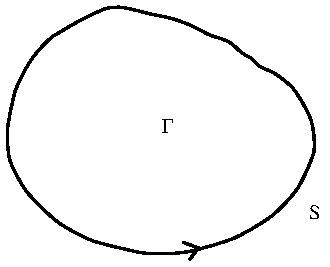
\includegraphics[width=0.3\linewidth]{./figures/lagrangian/vorticityCirculation.pdf}
	\caption{Circulation of the fluid}
	\label{fig:vorticityCirculation}
	\end{figure}

 
\subsection{Velocity-vorticity formulation of the Navier-Stokes equations}
The governing equation of the vortex particle method is velocity-vorticity $\mathbf{u}-\omega$ formulation of the Navier-Stokes equations \cite{Cottet2000a}. The 2-D incompressible Navier-Stokes momentum equation is given as

	\begin{equation}
	\frac{\partial \mathbf{u}}{\partial t} + \mathbf{u}\cdot\nabla\mathbf{u} = - \frac{1}{\rho} \nabla p + \nu \nabla^2\mathbf{u},
	\label{eq:mom}
	\end{equation}

relating the velocity field $\mathbf{u}\left(\mathbf{x},t\right)$ to the pressure field $\mathbf{p\left(\mathbf{x},t\right)}$, the kinematic viscosity $\nu$ and density $\rho$. Furthermore, we also have to satisfy the incompressibility constraint given as

	\begin{equation}
	\nabla\cdot\mathbf{u} = 0.
	\end{equation}

To attain the velocity-vorticity formulation, we should take the curl of the velocity-pressure $\mathbf{u}-p$ formulation of the Navier-Stokes equation. Taking the curl of the momentum equation \ref{eq:mom}, we get the vorticity transport equation

	\begin{equation}
	\frac{\partial \omega}{\partial t} + \mathbf{u}\cdot\nabla\omega = \nu \nabla^2 \omega,
	\end{equation}

which only relates the vorticity to the velocity enabling us to neglect the pressure field. Note that as we are dealing with the two dimensional flow, we neglected the stretching term. 


\subsection{Viscous splitting algorithm}
Vortex particle method was initially used to model the evolution of incompressible, inviscid flows. However, in order to simulate a real flow, we must also deal with the viscous behaviour of the fluid. Chorin \cite{Chorin1973} has shown that using the viscous splitting algorithm, it is possible to simulate a viscous flow. 

The viscous splitting algorithm is basically a fractional step method, where the viscous and the inviscid part of the transport equation is dealt in two subsequent steps, 

	\begin{itemize}
	\item Sub-step 1: convection
		\begin{equation}
		\frac{\partial\omega}{\partial t} + \mathbf{u}\cdot\nabla\omega=0;
		\label{eq:convectionEulerian}
		\end{equation}
		
	\item Sub-step 2: diffusion
		\begin{equation}
		\frac{\partial\omega}{\partial t} = \nu\nabla^2\omega.
		\label{eq:vsa2}
		\end{equation}
	
	\end{itemize}

The first sub-step of the evolution deals with the convection of the vorticity. Note that, by convection we imply the advection of the vorticity field where the diffusion process is neglected. The second sub-step is where we deals with the diffusion of the vorticity field. 

There are several advantage to this type of evolution. As the convection and diffusion are handled separately, there is minimum dispersion during the convection and furthermore, the is no restriction of the advection CFL number \cite{Wee2006}.

There are many ways of dealing with the diffusion of the vorticity field. During this project, we use a modified interpolation kernel \cite{Wee2006} that can simultaneously treat diffusion and remesh the vortex particles, see section \ref{sec:diffusionVM}.

%------------------------------------------------------------------------------------------------------
%------------------------------------------------------------------------------------------------------
%------------------------------------------------------------------------------------------------------
\section{Spatial Discretization: Generation of Vortex Blobs}
\label{sec:spatialDiscretization}

In order to deal with the vorticity field, we must first discretize the vorticity to vortex particles. Vortex blobs have been first introduced by Chorin and is a mollified particle carrying the local circulation. Vortex blobs describes a smooth vorticity field and are ideal because of it does not cause singularity issues when particles approach each other.

\todo{check for consistency, continuity}
\subsection{Biot-Savart law}

The velocity field can be decomposed using the Helmholtz decomposition, given as

	\begin{equation}
	\mathbf{u} = \mathbf{u}_{\omega} + \mathbf{u}_{\phi},
	\label{eq:helmholtz}
	\end{equation}

where $\mathbf{u}_{\omega}$ is the rotational component of the velocity and $\mathbf{u}_{\phi}$ is the irrotational component. solenoidal and potential velocity respectively. In an unbounded flow we have $\mathbf{u}_{\phi}$ equal to the free-stream velocity $\mathbf{u}_{\infty}$. For bounded flow, we must include the presence of the body, see section \ref{sec:boundaryConditions}.
	
The velocity can be related to the vorticity using the Biot-Savart law

	\begin{equation}
	\mathbf{u}_{\omega} = \mathbf{K}\star\omega,
	\end{equation}
	
where the $\star$ represents convolution of the 2-D kernel $\mathbf{K}$ given by

	\begin{equation}
	\mathbf{K} = \frac{1}{2\pi\left|\mathbf{x}\right|^2}\left(-x_2,x_1\right).
	\label{eq:GreensKernel}
	\end{equation}
	
\subsection{Discrete form of vorticity field}
The spatial discretization of the fluid domain is done through $N$ quadrature points. With the Biot-Savart law, we can treat these quadratures are discrete particles carrying the local quantities. The discrete vorticity field is given as

	\begin{equation}
	\omega\left(\mathbf{x},t\right) \simeq \omega^h\left(\mathbf{x},t\right) = \sum_{p}\alpha_p\left(t\right)\delta \left[\mathbf{x}-\mathbf{x}_p\left(t\right)\right],
	\end{equation}

where $\alpha_{p}$ is the estimate of the circulation around the particle $\mathbf{x}_p$ with core size $\sigma$. We must not that $\omega^h$ is an approximately equal to $\omega$ of the fluid due to the discretization.

The discrete form of the velocity is therefore written as

	\begin{equation}
	\mathbf{u} \simeq \mathbf{u}^h = \sum_p \mathbf{K}\left[\mathbf{x}-\mathbf{x}_p\left(t\right)\right]\alpha_p\left(t\right).
	\end{equation}
	
Thus the discrete vorticity field is an $N$-body problem inducing velocity on each and implicitly evolving the vorticity field. This is one of the advantage of the vortex particle method as there are many ways to efficiently treat the problem. The $N$-body problem can be parallelized and can be accelerated using fast summation methods such as FMM, see \ref{sec:sat}.
	
However, like all $N$-body problem, equation \ref{eq:GreensKernel} has a singularity when the particles approach each other and can result in numerical instability. To overcome this we can mollify the kernel, removing the singularity.

\subsection{Convection of vortex blobs}

In the discrete of the convection equation \ref{eq:convectionEulerian} of the viscous-splitting algorithm, the is solved as system of ODEs, where

	\begin{equation}
	\frac{\mathrm{d}\mathbf{x}_p}{\mathrm{d}t} = \mathbf{u}\left(\mathbf{x}_p\right),
	\end{equation}
with
	\begin{equation}
	\frac{\mathrm{d}\alpha_p}{\mathrm{d}t} = 0.
	\end{equation}

As the diffusion is done at the next sub-step, we have to ensure that the circulation is conserved.


\subsection{Mollified vortex kernels}

A vortex particle with a mollified core, non-zero core-size, is referred to as vortex blobs. The advantage of the vortex blobs is that the with a smooth distribution of the vorticity, the singularity disappears and so numerical instability does not happen when blobs get too close to each other. An ideal choice for a cutoff function is a Gaussian distribution, figure \ref{fig:gaussianDistribution}.

	\begin{figure}[t]
	\centering
	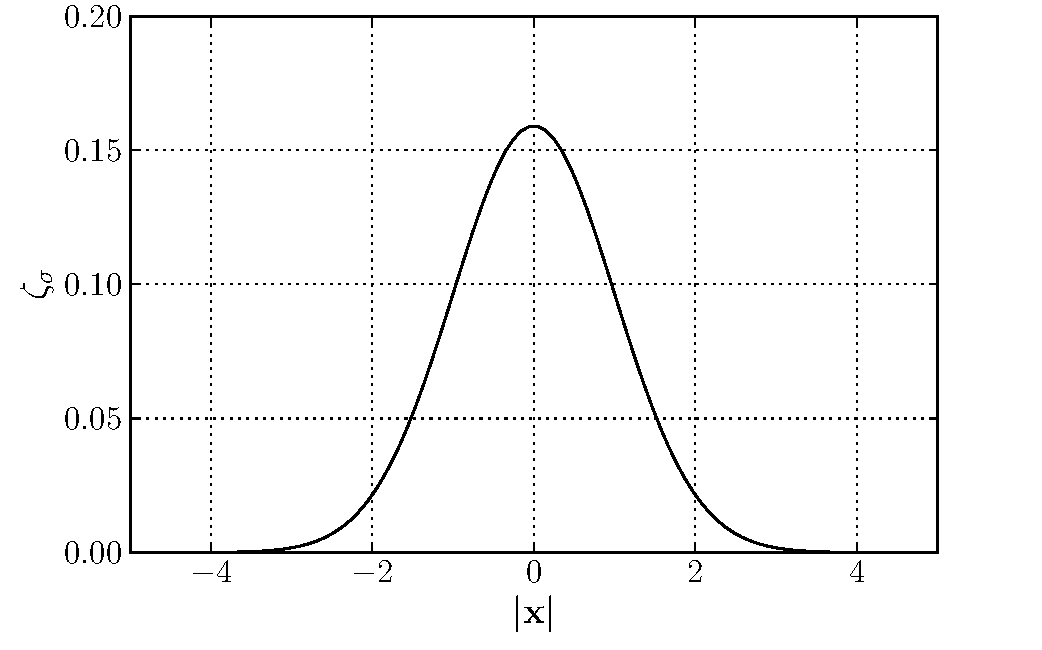
\includegraphics[width=0.7\textwidth]{figures/lagrangian/gaussianKernel.pdf}
	\caption{Vortex blob with Gaussian distribution: [$k=2$, $\sigma=1.0$]}
	\label{fig:gaussianDistribution}
	\end{figure}

Gaussian kernels satisfy the requirement for smooth distribution ad decays quickly and is defined as
	
	\begin{equation}
	\zeta_{\sigma} = \frac{1}{k\pi\sigma^2}\exp\left(\frac{-\left|\mathbf{x}\right|}{k\sigma^2}\right),
	\end{equation}

where $k$ is 1, 2 or 4 and determines the width of the kernel, $\sigma$ is core-size of the blob. Note that smoothing function is chosen such that $\int \zeta = 1$, ensuring the conservation of circulation when mollified. So, using a smooth cut-off function $\zeta_{\sigma}$, the mollified kernel $\mathbf{K}_{\sigma}$ is given as 

	\begin{equation}
	\mathbf{K}_{\sigma} = \mathbf{K} \star \zeta_{\sigma}.
	\end{equation}

The mollified vorticity field, represented by vortex blobs is given as

	\begin{equation}
	\omega^h\left(\mathbf{x},t\right) = \sum_p \alpha_p\left(t\right)\zeta_{\sigma}\left[\mathbf{x}-\mathbf{x}_p\left(t\right)\right],
	\label{eq:mollifiedVorticityField}
	\end{equation}

now representing the mollified vorticity field and equivalently, the mollified velocity field is given as

	\begin{equation}
	\mathbf{u}^h\left(\mathbf{x},t\right) = \sum_p \mathbf{K}_{\sigma}\left[\mathbf{x}-\mathbf{x}_p\left(t\right)\right]\alpha_p\left(t\right).
	\end{equation}

Koumoutsakos and Chorin \cite{Cottet2000a}, have shown that for proper communication between the particle, the particle needs to overlap,

	\begin{equation}
	\mathrm{overlap} = \frac{\sigma}{h},
	\end{equation}

	\begin{figure}[t]
	\centering
	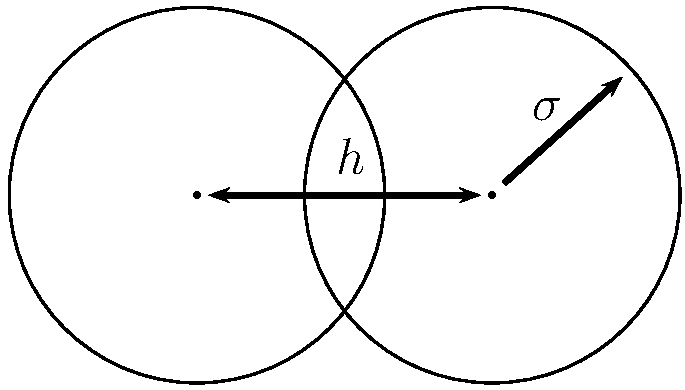
\includegraphics[width=0.4\textwidth]{figures/lagrangian/blobOverlap.pdf}
	\caption{Vortex blob with overlap $\sigma/h$}
	\label{fig:blobOverlap}
	\end{figure}

	
where $h$ is the nominal particle spacing, figure \ref{fig:blobOverlap}. If the particles fail to overlap, vortex blobs will also fail to recover the vorticity field. Such problems occurs when blobs are clustered due to high flow strain, leading to lagrangian grid distorting and must be treated, see section \ref{subsec:remeshing}.


\subsection{Vortex blob initialization}

Now the question arises on how to initialize the particle's circulation strengths $\alpha_p$. A common approach that is used is to estimate the particles strength is to say that

	\begin{equation}
	\alpha_p = \omega_p\cdot h^2.
	\label{eq:particleCirculationAssignment}
	\end{equation}

This might seem like a valid assumption as the circulation of a given area is the integral of the vorticity in the area, equation \ref{eq:definitionOfCirculation}, however this is no longer valid when regularizing the vorticity field using mollified gaussian kernels, equation \ref{eq:mollifiedVorticityField}. Barba and Rossi \cite{Barba2010}, has described this problem as gaussian blurring of the original vorticity field. Even though the particle have acquired the correct circulation strengths (i.e the local property), when evaluating the mollified vorticity field, we see that there is a mismatch in the evaluated vorticity field, figure \ref{fig:particleInitialization}. 


	\begin{figure}[t]
	\centering
	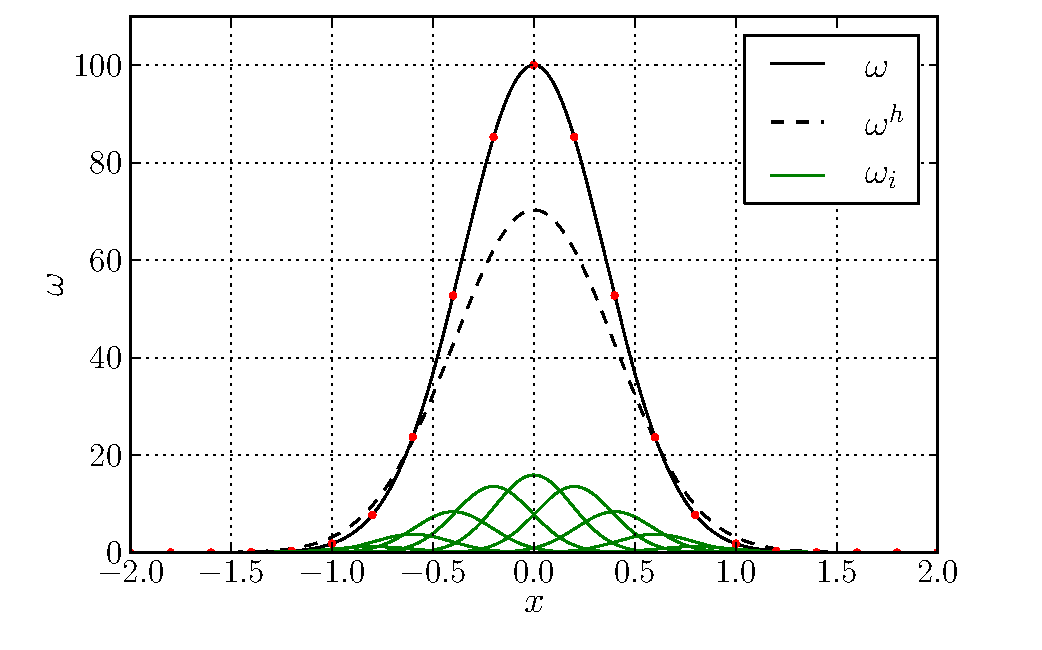
\includegraphics[width=0.7\textwidth]{figures/lagrangian/particleInitialization.pdf}
	\caption{Mollified vorticity field of an arbitrary vorticity function with $\mathrm{overlap}=1.0$, $\sigma=0.19$, $h=0.19$. Vortex blob strength has been assigned by equation \ref{eq:particleCirculationAssignment}, sampling at exact vorticity [{\color{plotRed}{$\bullet$}}, red dot]. Figure depicts exact vorticity distribution $\omega$ [---, solid], vorticity field of each blob $\omega_i$ [{\color{darkgreen}{---}}, green dashed], the mollified vorticity field $\omega^h$ [- -, dashed].  }
	\label{fig:particleInitialization}
	\end{figure}

Another way of viewing this characteristic is say the conservation of circulation is only valid globally, but not locally. A common standard for recovering the initial vorticity field is perform the Beale's method \cite{Beale1988}.

\subsubsection*{Beale's Iterative Method}

The Beale's method is particle circulation processing scheme where the circulation of the particles are modified such that the mollified vorticity field matches the indented vorticity field. The recovery of the vorticity field is done by performing a discrete deconvolution,

	\begin{equation}
	\sum_j^N \beta_j \zeta_{\sigma}\left(\mathbf{x}_i-\mathbf{x}_j\right) = \omega_i,
		\end{equation}

where $\beta_j$ is the circulation of the particles at positions $\mathbf{x}_j$ such that it matches the exact vorticity $\omega_i$ at the position $\mathbf{x}_i$ that we are evaluating.  As we are try to solve for a $N$ unknown problem, we must set up a $N$ system of equations. Multiplying both sides with the area associated to the blobs, we get

	\begin{equation}
	\mathbf{A}_{ij} \beta_j = \alpha_i^{\mathrm{exact}},
	\end{equation}
	
where

	\begin{equation}
	\mathbf{A}_{ij} = \zeta_{\sigma}\left(\mathbf{x}_i - \mathbf{x}_j\right) \cdot h^2
	\end{equation}

is a $N \times N$ matrix containing the weights of the influence of each particle on each other. This matrix can be constructed by setting the $\Gamma$ to one and determine the induced vorticity on each other. Furthermore, we see that it is not feasible to directly invert the matrix when we have large set of blobs but most importantly as the matrix $\mathbf{A}$ is severly ill-conditioned \cite{Speck2011a}, it should not be directly inverted. Beale's proposition to this problem was to iteratively solve for the solution,

	\begin{equation}
	\beta_{j}^{n+1} = \alpha_i + \beta_i^n - \mathbf{A}_{ij}\cdot\beta_j^n
	\end{equation}
	
We see that with just two iterations, the error between the mollified and exact vorticity field reduces drastically, figure \ref{fig:bealesCorrection}. Koumoutsakos and Cottet \cite{Cottet2000a}, had shown that there was a drastic improvement in the velocity with just two to three iterations. However, we see that the cell vorticity of the blobs, directly evaluated from the particle strengths, equation \ref{eq:particleCirculationAssignment}, are more peaky and no longer matches the exact vorticity. 

During the hybrid coupling algorithm, we see that this is the central source of coupling error between the eulerian and the lagrangian method, section \ref{}. When performing the hybrid coupling, we need to recover the vorticity field transfered from the eulerian domain to the lagrangian domain in every step. So, beale's correction is not a viable solution for the hybrid method. Thus there is a need for an alternate method of recovering the vorticity field.

\todo{add the reference to hybrid}

	\begin{figure}[t]
	\centering
	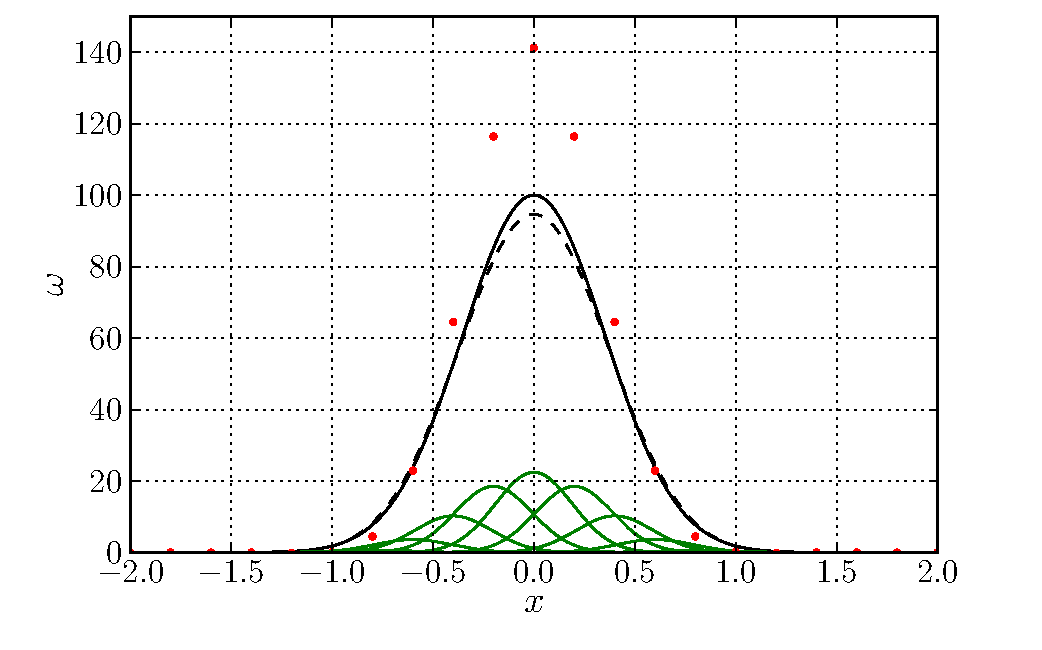
\includegraphics[width=0.7\textwidth]{figures/lagrangian/bealesCorrection.pdf}
	\caption{Mollified vorticity field after two Beale's iteration, $\mathrm{overlap}=1.0$, $\sigma=0.19$, $h=0.19$. Figure depicts exact vorticity distribution $\omega$ [---, solid], vorticity field of each blob $\omega_i$ [{\color{plotGreen}{---}}, green dashed], the mollified vorticity field $\omega^h$ [- -, dashed].  }
	\label{fig:bealesCorrection}
	\end{figure}



\subsubsection{Convergence of particle discretization}

An alternate, temporary method to reduce the gaussian blurring of the vorticity field is to reduce the overlap (i.e. increase the overlap ratio) of the vortex blobs and to the increase the spatial resolution.
	
\begin{figure}[b]
        \centering
        \begin{subfigure}[b]{0.5\textwidth}
                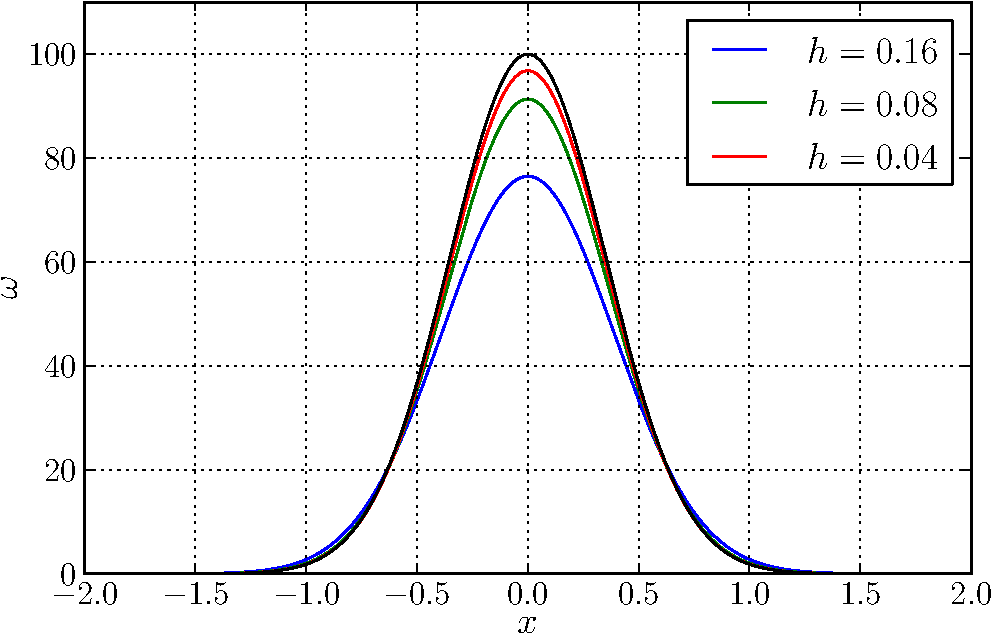
\includegraphics[width=\textwidth]{figures/lagrangian/betterInitialization_h-crop.pdf}
                \caption{Convergence of $h$ with $\mathrm{overlap} = 1.0$}
                \label{fig:convergenceOfBlobsH}
        \end{subfigure}%
        ~ %add desired spacing between images, e. g. ~, \quad, \qquad etc.
          %(or a blank line to force the subfigure onto a new line)
        \begin{subfigure}[b]{0.5\textwidth}
                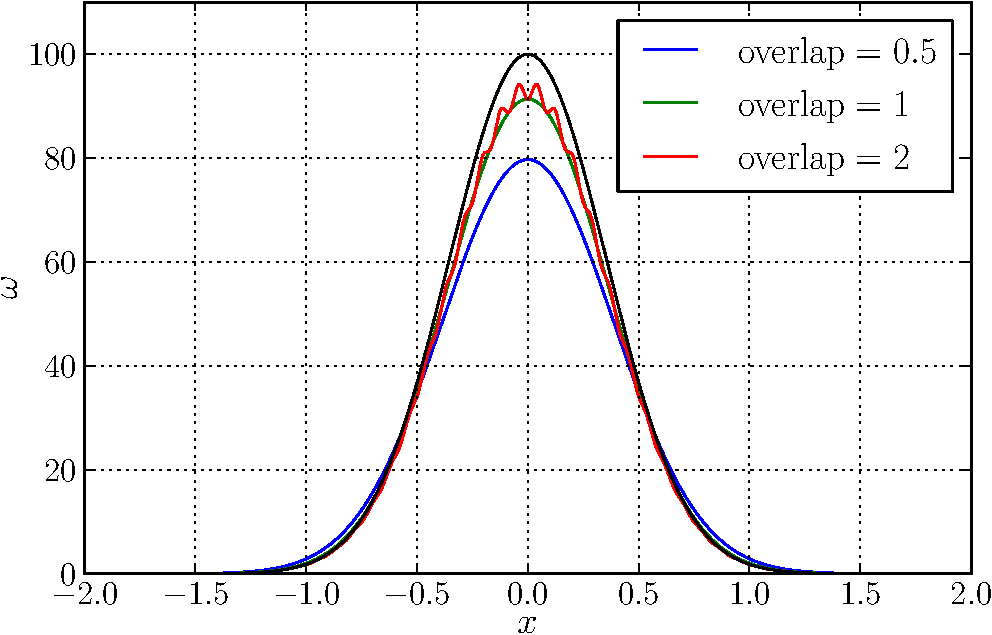
\includegraphics[width=\textwidth]{figures/lagrangian/betterInitialization_overlap-crop.pdf}
                \caption{Convergence of $\mathrm{overlap}$ with $h = 0.08$}
                \label{fig:convergenceOfBlobsOverlap}
        \end{subfigure}
        \caption{Convergence of vorticity by modifying the spatial resolution. Figure depicts exact vorticity field $\omega$ with [---, black] and various resolutions.}
        \label{fig:convergenceOfSpatialResolution}
\end{figure}	

Figure \ref{fig:convergenceOfSpatialResolution} shows mollified vorticity field results from modifying the spatial resolution parameters. Figure \ref{fig:convergenceOfBlobsH} shows the convergence of the mollified vorticity field $\omega^h$ to the exact vorticity field $\omega$ by reducing the nominal particle spacing $h$. The blobs have $\mathrm{overlap} = 1$ and so the blob core-size $\sigma$ is equal to $h$. We see that as you reduce the size of the blob and increase the number of particles, the mollified vorticity converges to the exact vorticity. Therefore, an alternate method of reducing the gaussian blurring is to increase the spatial resolution.

Furthermore, we could also adjust the $\mathrm{overlap}$ of the blobs, figure \ref{fig:convergenceOfBlobsOverlap}. The $\sigma$ and $h$ of the blob is $0.08$ and we see that increasing overlap number (i.e reducing the overlap), helps us to recover the original vorticity field. However, as explained by Koumoutsakos \cite{Cottet2000a}, if the overlap is too low, we lose the smooth recovery of the vorticity field. This is apparent when $\mathrm{overlap} = 2.0$, where we see that the mollified vorticity field is fluctuation.

Therefore, for the hybrid coupling, we set $\mathrm{overlap} = 1.0$ and maximize the spatial resolution at the coupling zone. 

\subsection{Remeshing scheme: Treating lagrangian grid distortion}
\label{subsec:remeshing}
%
%%------------------------------------------------------------------------------------------------------
%%------------------------------------------------------------------------------------------------------
%%------------------------------------------------------------------------------------------------------

During the convection step, we see that another source of error in the vorticity field is the lagrangian grid distortion. As we have seen before, when the vortex blobs fails to overlap, we are no longer able to reconstruct the correct the vorticity field, figure \ref{fig:convergenceOfBlobsOverlap}. During the convection, due to the high strains in the fluid, the vortex blobs tent to clump together and creates regions where no vortex blobs are found, reducing the overlap of the blobs, figure \ref{fig:distortion}. 

%\begin{figure}[t]
%        \centering
%        \begin{subfigure}[b]{0.45\textwidth}
%                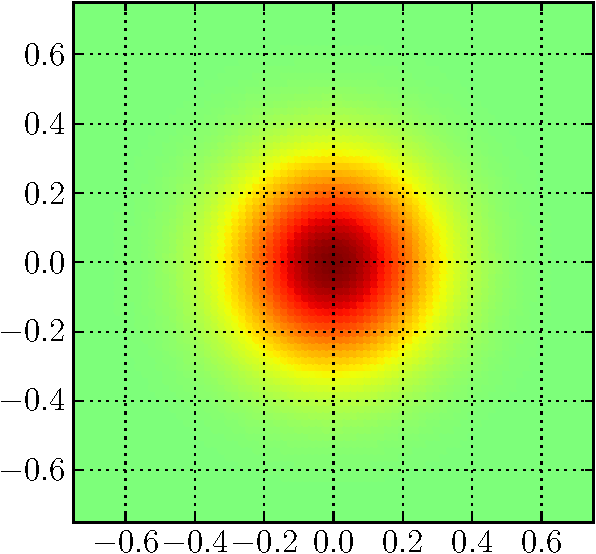
\includegraphics[width=\textwidth]{figures/lagrangian/distortion_a-crop.pdf}
%                \caption{$t = 0$}
%                \label{fig:distortion_a}
%        \end{subfigure}%
%        \qquad %add desired spacing between images, e. g. ~, \quad, \qquad etc.
%          %(or a blank line to force the subfigure onto a new line)
%        \begin{subfigure}[b]{0.45\textwidth}
%                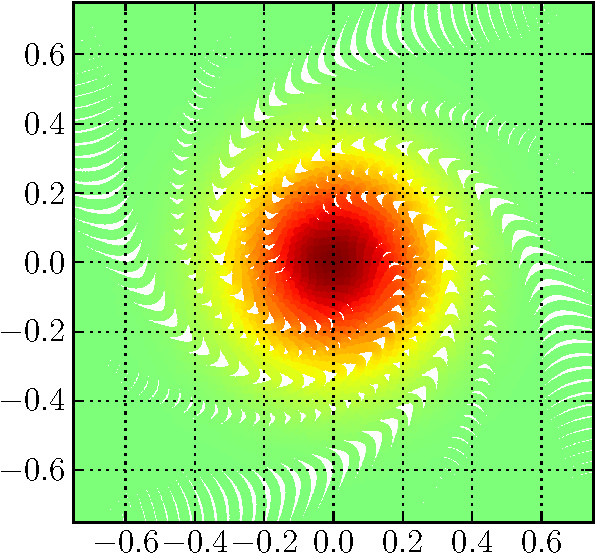
\includegraphics[width=\textwidth]{figures/lagrangian/distortion_b-crop.pdf}
%                \caption{$t = 10$}
%                \label{fig:distortion_b}
%        \end{subfigure}
%        \caption{Lagrangian distortion of the vortex blobs after 100 steps. The initial vorticity field $\omega\left(\mathbf{x},0\right) = \exp\left(-12\left|\mathbf{x}\right|\right)$ with $\Delta t = 0.1$, $\sigma=0.02$ and $\mathrm{overlap} = 1.0$. Figure depicts the initial and the final distribution of the vortex blobs.}
%        \label{fig:distortion}
%\end{figure}

	\begin{figure}[t]
	\centering
	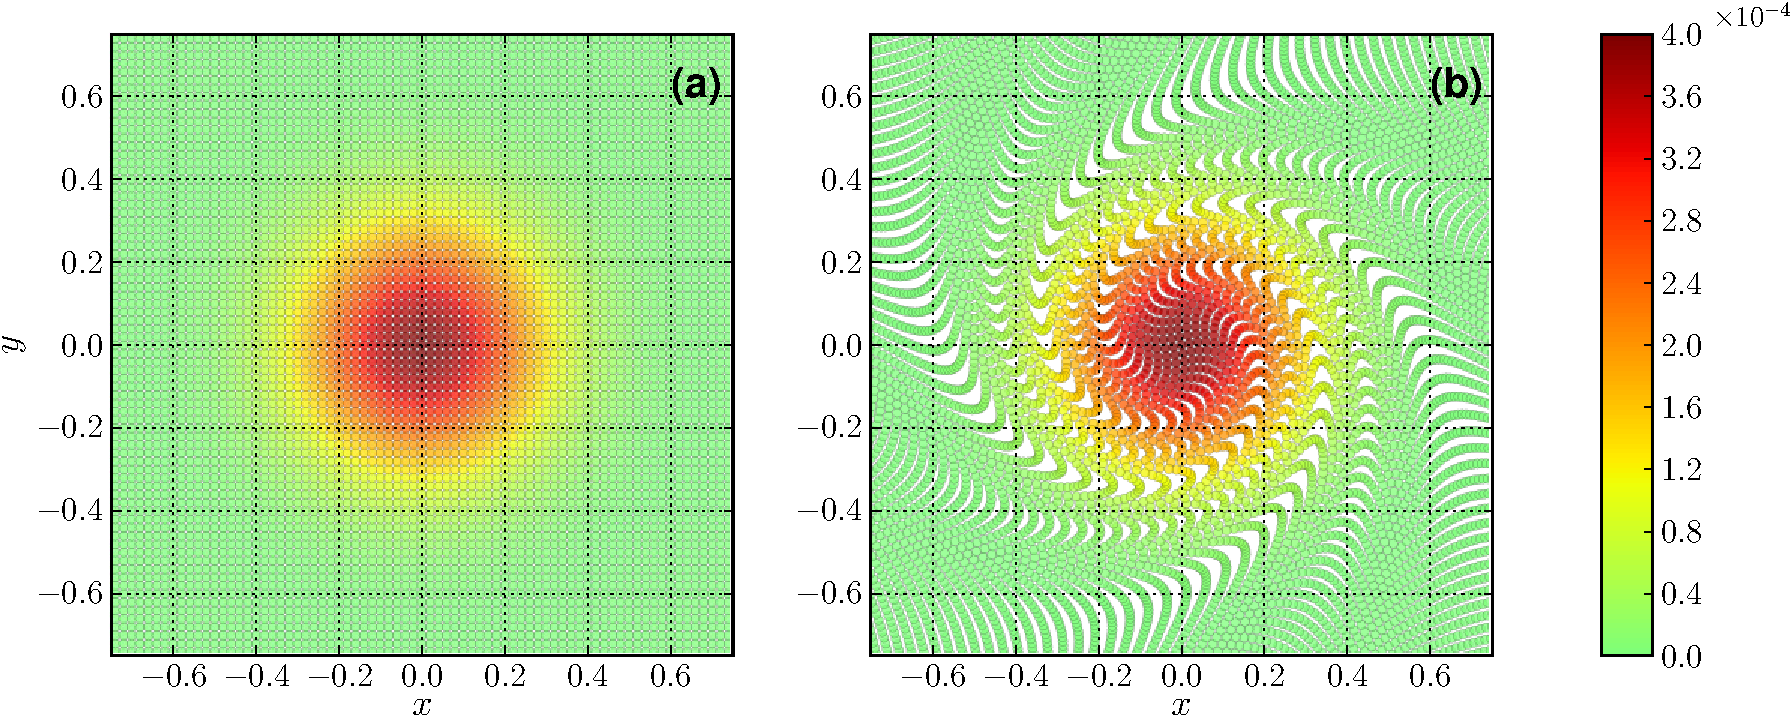
\includegraphics[width=0.9\textwidth]{figures/lagrangian/distortion-crop.pdf}
    \caption{Lagrangian distortion of the vortex blobs after 100 steps. The initial vorticity field $\omega\left(\mathbf{x},0\right) = \exp\left(-12\left|\mathbf{x}\right|\right)$ with $\Delta t = 0.1$, $\sigma=0.02$ and $\mathrm{overlap} = 1.0$. Figure depicts $\textbf{(a)}$ the initial and $\textbf{(b)}$ the final distribution of the vortex blobs.}
    \label{fig:distortion}
	\end{figure}


We see that due to clustering of the vortex blobs, it fails to reproduce the correct vorticity field. A common strategy to overcome this problem is to remesh the vortex blobs to a uniform grid, so that we have a continuous vorticity field.

However, when transfering the vorticity from the old deformed grid to the new lagrangian uniform grid, we must satisfy the conservation laws of vorticity field. The interpolation methods is based on the conservation of linear impulse which directly implies the conservation of the total circulation \cite{Cottet2000a}. The transfer of the particle strengths is given as, 

	\begin{equation}
	\alpha_p = \sum_q\tilde{\alpha}_q W \left(\frac{x_p - \tilde{x}_q}{h}\right),	
	\end{equation}

where the strengths of the particles $\tilde{\alpha}_q$ of the distorted lagrangian grid $\tilde{x}_q$ is transfered to the regular lagrangian grid $x_p$ using the interpolation kernel, weighted $W$, giving us the remeshing particle strengths $\alpha_p$. The transfer of strengths of one particles to it's interpolation nodes can be seen in figure \ref{fig:interpolationGrid}.


	\begin{figure}[t]
	\centering
	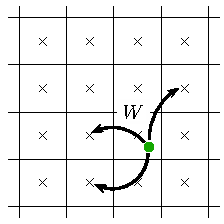
\includegraphics[width=0.4\textwidth]{figures/lagrangian/interpolationGrid.pdf}
	\caption{Remehsing of vortex blob ({\color{plotGreen}{$\bullet$}}, green) on the uniform grid defined by the $\left(4\times4\right)$ 2-D stencil.}
	\label{fig:interpolationGrid}
	\end{figure}

\subsubsection*{$\mathbf{M}^\prime_4$ interpolation kernel}
For lagrangian problem, we use the efficient interpolation kernel that has been used to reconstruct a smooth distribution interpolation, the $\mathrm{M}^{\prime}_4$ interpolation kernel, introduced by Monaghan \cite{Monaghan1985}. In one dimension it is given as,

	\begin{equation}
	{\mathrm{M'}_4}\left( {\xi} \right) =
	  \begin{cases}
	   {1 - \frac{{5{\xi ^2}}}{2} + \frac{{3{{\left| \xi  \right|}^3}}}{2}} & {\left| \xi \right|} < 1, \\
	   \frac{1}{2}{\left( {2 - \left| \xi  \right|} \right)^2}\left( {1 - \left| \xi  \right|} \right) & 1 \le {\left| \xi \right|} < 2,\\
	   0 & 2 \le \left| \xi \right|,
	  \end{cases}
	\label{eq:interpKernel}
	\end{equation}

where 

	\begin{equation}
	\xi = \frac{x_{\nu} - x_i}{h}
	\label{eq:xiEquation}
	\end{equation}

is the scale relative position of the particle $x_{\nu}$ to the $i^{\mathrm{th}}$ interpolation node $x_i$. The $\mathrm{M'}_4$ is a third-order accurate piecewise smooth B-spline kernel, where $m = 4$ giving it 4 support nodes, figure \ref{fig:interpolationKernel}. For the two dimensional problem that we have, the 2-D interpolation formula is simply tensor product of the 1-D interpolation kernel equation \ref{eq:interpKernel}, and results in $4^2 = 16$ support nodes, figure \ref{fig:interpolationGrid}.

	\begin{figure}[t]
	\centering
	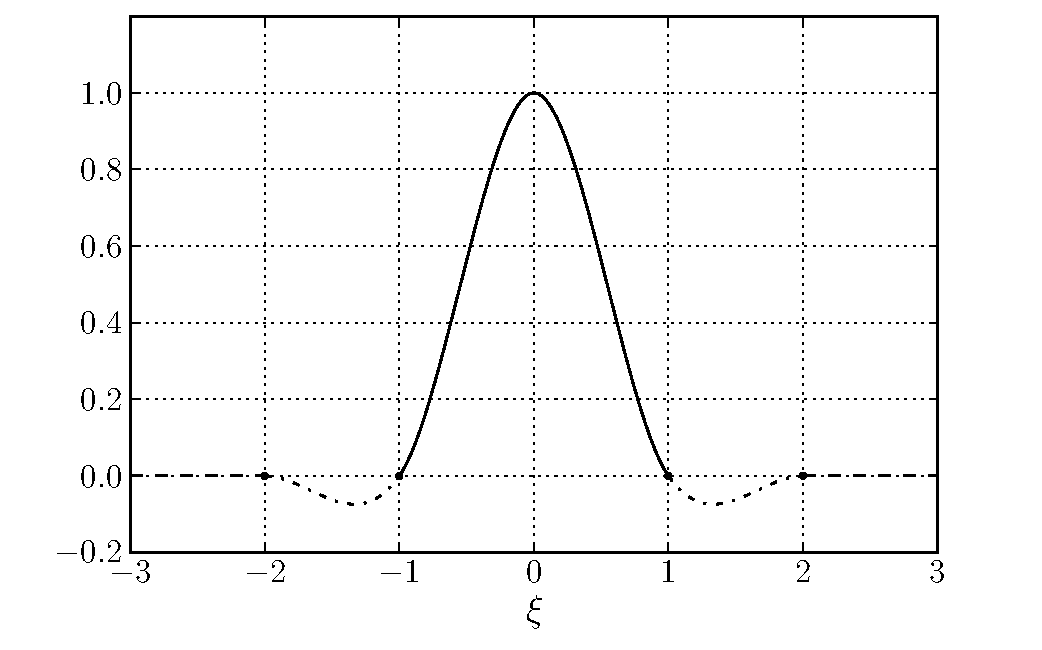
\includegraphics[width=0.7\textwidth]{figures/lagrangian/interpolationKernel.pdf}
	\caption{Monaghan's \cite{Monaghan1985} third-order peicewise smooth B-spline kernel, $M'_4$}
	\label{fig:interpolationKernel}
	\end{figure}

The interpolation kernel achieves the third-order accuracy as it also conserves the linear and the angular momentum of the vortex. Koumoutsakos \cite{Koumoutsakos1997} has investigated the drawback of the employing the remeshing strategy and have shown that there is approximately $4\%$ decay in enstrophy of the flow due to sub-grid dissipation. Note that enstrophy $ \mathcal{E}$, is defined as

	\begin{equation}
	\mathcal{E} = \frac{1}{2}\int_S \omega^2 dS
	\end{equation}
	
and is directly related to the kinetic energy of the fluid and gives and insight in the energy production and the dissipation of the fluid. Enstrophy is especially useful in turbulence flow investigation as it helps describe the energy cascade of the fluid.		

\section{Diffusion of Vortex Methods}
\label{sec:diffusionVM}

So far, we have dealth with unbounded Euler flow, where we disregarded the viscosity of the flow. However, for real flow we must take in account of the diffusion of the vorticity. Chorin's approach to deal with the viscous term was to employ the viscous splitting algorithm. The flow is segregated to inviscid and viscous component and during the second sub-step we deal with the diffusion of the vorticity, equation \ref{eq:vsa2}. The equation can again be solved as a system of ODEs, similar to the convection step, where we say,

	\begin{equation}
	\frac{\mathrm{d}\mathbf{x}_p}{\mathrm{d}t} = 0,
	\end{equation}
with
	\begin{equation}
	\frac{\mathrm{d}\alpha_p}{\mathrm{d}t} = \nu\Delta\alpha_p.
	\end{equation}

Therefore in the diffusive step, we fix the position of the vortex blobs and only have to modify the strengths of the particles to mimic the diffusion process. Chorin initially employed a random walk method, which generates and disperse vorticity using pseudo-random number algorithm \cite{Chorin1973}. However, this method suffers some limitations in accuracy. Since then \printAcron{Particle Strength Exchange}{PSE} method \cite{Degond1989}, has been a common approach that has been used to treat diffusion.

\subsubsection*{Particle Strength Exchange}
The Particle Strength Exchange method, first proposed by Mas-Gallic \cite{Degond1989}, showed that diffusion can be treated for a particle method isotropic and anisotropic viscosity by approximating the diffusion operator (laplacian) with an integral operator and discretizing the operator using particles. The PSE can be seen as circulation correction method, where during the diffusion step of the viscous splitting algorithm, the strengths of the particle are corrected such that it accounts for the diffusion.
 
\subsubsection*{Vortex Redistribution Method}
An alternative method to simulate the diffusion is to use the \printAcron{Vortex Redistribution Method}{VRM} \cite{Shankar1996}. The model simulates diffusion by distributing the fraction of circulation of the vortex blobs to each other satisfying the diffusion. The model is based on conserving the moments of the particles by satisfying a linear system of equations. The circulation of the particle are transfer to the nearby particles that are 

	\begin{equation}
	h_{\nu} = \sqrt{\nu\Delta t_d}
	\end{equation}

where $h_{\nu}$ is the diffusion distance and is directly related to the kinematic viscosity $\nu$ and the diffusive time-step $\Delta t_d$ of the simulation. Not that the diffusive time-step $\Delta t_d$ is equal to the convective time-step $\Delta t_c$ if the diffusion process is done during every time-step. However, we can easily adjust the diffusion time-step and perform diffusion at a multiple step of the convection.

This is vital as a VRM (and also the PSE) requires a search algorithm to determine the particles that are within the zone of influence. A direct evaluation required $\mathcal{O}\left(N^2\right)$ evaluation, however can be speed up to $\mathcal{O}\left(\log N\right)$ using search tree algorithm.

The downside of the this approach, as also for the standard remeshing approach is the global remeshing generates large computation data and scales with the number of particles $N$. Therefore for problems with large number of particles, a tree-structured remeshing would be more feasible strategy \cite{Winckelmans1996}.

\subsection{Modified remeshing for treating diffusion}
From further investigation of the VRM, we see that it is similar to remeshing strategy used to counter the lagrangian distortion during the convection process. Therefore Ghoniem and Wee \cite{Wee2006} has proposed to combine the remeshing and the diffusion. The application of this methodology was validated by Speck \cite{Speck2011a}. The diffusion is simulated by the modifying the interpolation kernel of the remeshing process. The key advantage of the modified remeshing method is that now it deals with the uniform remeshing grid helping us eliminating the computational expensive research requirement. The second advantage as shown by the authors is the simplicity. The method only requires a slight modification to the original remeshing tool.

During remeshing, the heat equation is satisfied by transferring the correct fraction of circulation to produce the proper amount of diffusion. The $\mathrm{M'}_4$ kernel was modified to treat the diffusion and is given by: 

\begin{equation}
{{{\rm{M'}}}_4}\left( {\xi ,c} \right) =
  \begin{cases}
   {1 - \frac{{5{\xi ^2}}}{2} + \frac{{3{{\left| \xi  \right|}^3}}}{2} - {c^2}\left( {2 - 9{\xi ^2} + 6{{\left| \xi  \right|}^3}} \right)} & {\left| \xi \right|} < 1, \\
   \frac{1}{2}{\left( {2 - \left| \xi  \right|} \right)^2}\left( {1 - \left| \xi  \right|} \right) - {c^2}{\left( {2 - \left| \xi  \right|} \right)^2}\left( {1 - 2\left| \xi  \right|} \right) & 1 \le {\left| \xi \right|} < 2,\\
   0 & 2 \le \left| \xi \right|,
  \end{cases}
\label{eq:modInterpKernel}
\end{equation}

where 

\begin{equation}
c^2 = \frac{\nu \Delta t_d}{h^2},
\label{eq:c2}
\end{equation}

and corresponds to the transfer quantity for diffusion. The addition terms in the interpolation kernel accounts for the diffusion process. When $c \rightarrow 0$, the interpolation kernel turns to the classical non-diffusion kernel. 

Similar to the VRM, we can perform the remeshing at a given multiple step $k_d$ of the convection step. However, we have an additional constraint on the diffusion time-step $\Delta t_d$, equation \ref{eq:c2}. Wee and Ghoniem \cite{Wee2006} also investigated the error growth and the stability properties of the interpolation kernel in the Fourier space and have determined that for $\mathrm{M'}_4$ interpolation kernel, we must satisfy

\begin{equation}
\frac{1}{6} \le c^2 \le \frac{1}{2}.
\label{eq:c2stability}
\end{equation}

to ensure amplification factor and the phase error does not grow. This will ensure the stability of the problem and will suppress any spurious oscillations and ensure that it is a non-negative interpolation kernel with non-negative redistribution fractions. 

However, we see that constraint on $c^2$ not only imposes a maximum $\Delta t_d$ but also a constraint on the minimum $\Delta t_d$. This means that in scenarios, the $\Delta t_d = k_d \cdot \Delta t_c$ and this might introduce sudden change in vorticity field. Therefore, during the coupling of the lagrangian and eulerian domains, we would like to diffuse the vorticity after every convection scheme.

\subsubsection*{Simple redistribution scheme}

The simple redistribution scheme based on the Shankar and Van Dommelen \cite{Shankar1996}, developed by Tutty \cite{2010arXiv1009.0166T}, makes it possible to remesh and diffuse the vorticity after every convection step, 

	\begin{equation}
	\alpha_i^{n+1} = \sum_k \alpha_k^n W_{ki}^n, 
	\end{equation}

where $W_{ki}^n$ is the fraction of circulation from vortex blob $k$ transferred to vortex blob $i$ by diffusion during the time step $n$. The fractions $W_{ki}^n$ are calculated by conserving vorticity, center of vorticity, linear, and angular momentum of the vortex blobs \cite{2010arXiv1009.0166T}. In two dimensional problem the redistribution fractions are simple tensors products of the $x,y$ one dimensional redistribution fractions,


	\begin{figure}[t]
	\centering
	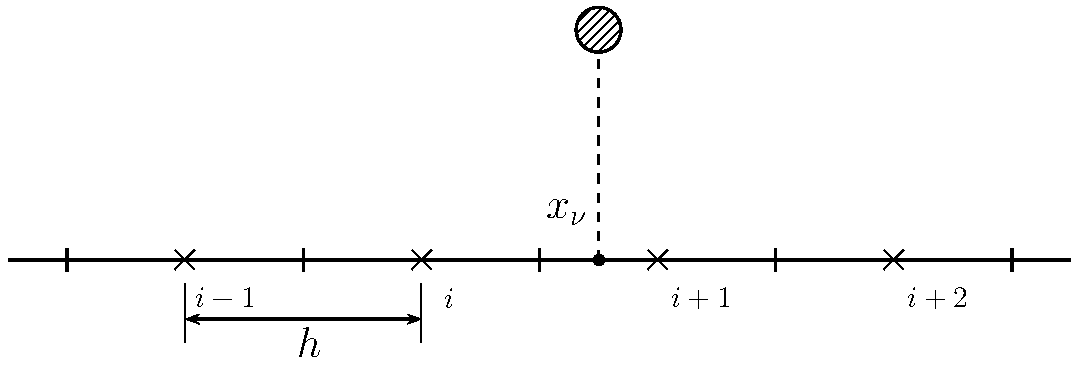
\includegraphics[width=0.7\textwidth]{figures/lagrangian/simpleRedistribution.pdf}
	\caption{One dimensional, Simple redistribution scheme, diffusing the vortex blobs to the four stencil points ($k=i-1,\dots,i+2$) with vortex blob positioned at $x_i \le x_{\nu} \le x_{i+1}$ and nominal blob spacing $h$.}
	\label{fig:simpleRedistribution}
	\end{figure}

	\begin{equation}
	W_{kl} = F_k G_l, \quad k = i-1,\cdots,i+2, \quad \l = j-1,\dots,j+2
	\end{equation}

giving it a 16 point stencil. The one-dimension redistribution fractions for $x$-direction is a linear combination of the two basis solution of the redistribution equation for conservations,

	\begin{equation}
	F_k = \left(1-\Delta\right)\cdot f_k + \Delta\cdot g_k, \quad k = i-1,\dots,i+2
	\end{equation}

having a four point stencil, figure \ref{fig:simpleRedistribution}. The basis solution of redistribution are 

	\begin{subequations}
	\begin{align}
	f_i &= 1 - 2\left(\frac{h_{\nu}}{h}\right)^2 - \xi^2\\
	f_{i-1} &= \frac{1}{2}\left(1-f_i-\xi\right)\\
	f_{i+1} &= \frac{1}{2}\left(1-f_i+\xi\right)
	\end{align}
	\end{subequations}
and 	
	\begin{subequations}
	\begin{align}
	g_{i+1} &= 1 - 2\left(\frac{h_{\nu}}{h}\right)^2 - \xi_1^2\\
	g_{i} &= \frac{1}{2}\left(1-g_{i+1}-\xi_1\right)\\
	g_{i+2} &= \frac{1}{2}\left(1-g_{i+1}+\xi_1\right)
	\end{align}
	\end{subequations}

where $\xi$ is given by equation \ref{eq:xiEquation}, $\xi_1 = \xi - 1$ are the distances between the $k^{\mathrm{th}}$ stencil nodes $x_k$ and the vortex blob that is to be diffused with $x_i \le x_{\nu} \le x_{i+1}$. Note, $f_k$ and $g_k$ is zero for all the other $k$. In the above equation, $h_{\nu}$ is the characteristic diffusion distance over the time $\Delta t_d$, 

	\begin{equation}
	h_{\nu} = \sqrt{\Delta t_d \cdot \nu}.
	\end{equation}
	
	
The only constraint imposed  for positive redistribution fraction is

	\begin{equation}
	\frac{h_{\nu}}{h} < \frac{1}{\sqrt{2}}.
	\end{equation}
	
giving us the maximum time-step size constraint of
	\begin{equation}
	\Delta t_d < \frac{h^2}{2\nu}.
	\end{equation}

So now, we are able to perform diffusion, together with the convection step (i.e $k_d = 1$).

\section{Boundary conditions at solid boundary}
\label{sec:boundaryConditions}

So far, we have only dealt with unbounded flow. During bounded flow simulation, we must impose addition constraint of the boundary to the simulation to simulate any flow about a geometry. From Helmholtz decomposition, we can have decompose the velocity field to the rotation and the irrotation component, equation \ref{eq:helmholtz}. With the Helmholtz decomposition, we can use the potential component to prescribe the boundary conditions at the solid wall boundary,
	\begin{equation}
	\mathbf{u}_{\phi} = \nabla\Phi.
	\end{equation}

The incompressibility constraint results in a Laplace's equation for the potential field and unique solution is obtained by enforcing the wall boundary conditions,
	\begin{equation}
	\mathbf{u}_b\cdot\mathbf{\hat{n}} = \left(\mathbf{u}_{\omega} + \nabla\Phi\right) \cdot \mathbf{\hat{n}},
	\label{eq:potentialBC}
	\end{equation}
and is defined as enforcing the no-through flow at the solid boundary wall, moving at $\mathbf{u}_b$. Note that the $\mathbf{\hat{n}}$ is the normal vector of the solid boundary. A classical approach for determine the solution to the Laplace's equation is by Green's function formulation. This approach required a singularity distribution over the body resulting in the appropriate boundary condition. Doublets and/or source panels are used to attain the required potential such that equation \ref{eq:potentialBC} is satisfied.

\subsubsection{Linked boundary conditions}

However Koumoutsakos, Leonard and Pepin \cite{Koumoutsakos1994b}, have suggested to enforce the boundary conditions through vortex sheets. The alternative approach of enforcing the solid boundary condition is not to decompose the velocity field into potential and rotational but to consider the solid boundary as an extension of the vorticity field through vortex sheets $\gamma$, figure \ref{fig:noSlipVorticityField}. Due to the non-zero tangential velocity at the surface, a sudden discontinuity in the velocity field can be considered as vortex sheet. Therefore, now to enforce the boundary conditions of the solid wall, we must satisfy the no slip velocity at the boundary,
	\begin{equation}
	\mathbf{u}\cdot\mathbf{\hat{s}} = \mathbf{u}_b\cdot\mathbf{\hat{s}}.
	\end{equation}

Koumoutsakos \cite{Koumoutsakos1993} only relies on the vortex sheet to enforce the no-slip velocity as no-slip boundary condition directly satisfies the no-through boundary conditions, also known as the linked boundary conditions. This was also proven by Shiels \cite{Shiels1998} and further investigated by Cooper, Mar and Barba \cite{Cooper2009b} and shown that vortex sheet is the only necessary singularity element required to satisfy both the boundary conditions. Therefore, enforcing the no-slip boundary condition directly satisfies the no-through constraint at the surface.
	\begin{figure}[t]
	\centering
	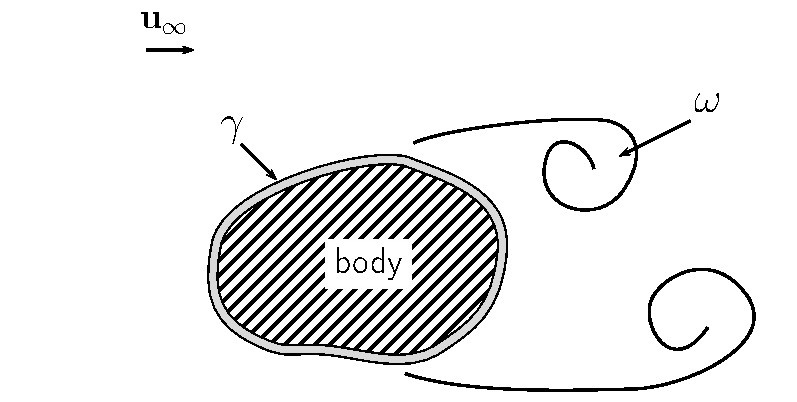
\includegraphics[width=0.6\textwidth]{figures/lagrangian/noSlipVorticityField.pdf}
	\caption{Extended vorticity field consisting of vorticity in the fluid and vortex sheet distribution around the body.}
	\label{fig:noSlipVorticityField}
	\end{figure}

\subsection{Boundary integral equations}
Thus the decomposed velocity field can be summarized as
	\begin{equation}
	\mathbf{u} = \mathbf{u}_{\omega} + \mathbf{u}_{\gamma} + \mathbf{u}_{\infty}
	\end{equation}
where the $\mathbf{u}_{\gamma}$ denotes the velocity filed induced by the vortex sheet. Applying the no-slip boundary conditions, we can say that
	\begin{equation}
	\left(\mathbf{u}_{\mathrm{ext}} + \mathbf{u}_{\gamma}\right)\cdot\mathbf{\hat{s}} = \mathbf{u}_b \cdot \mathbf{\hat{s}}
	\label{eq:kinematicBCofVSOutside}
	\end{equation}
where $\mathbf{u}_{\mathrm{ext}} = \mathbf{u}_{\omega} + \mathbf{u}_{\infty}$ is the velocity field induced from domain external of the body and the vortex sheet. For the tangential boundary condition, for a well-conditioned system of equations, the induced velocity from the vortex sheet can be summarized as  
	\begin{equation}
	\left(\mathbf{u}_{\mathrm{ext}} - \mathbf{u}_b\right) \cdot \mathbf{\hat{s}} = \mathbf{u}_{\gamma}\cdot\mathbf{\hat{s}}.
	\label{eq:kinematicBCofVS}
	\end{equation}

The equation states that underneath the vortex sheet, we must have a vortex sheet inducing the velocity field $\mathbf{u}_{\gamma}$ to counter the slip velocity $\mathbf{u}_{\mathrm{slip}} = \left(\mathbf{u}_{\mathrm{ext}} - \mathbf{u}_b\right)$ such that we satisfy the no-slip kinematic boundary conditions. Note that, $\mathbf{u}_{\gamma}$ of equation \ref{eq:kinematicBCofVS}, is negative of equation \ref{eq:kinematicBCofVSOutside} as we looking under the vortex sheet. Koumoutsakos \cite{Koumoutsakos1993}, expressed the relation of the vortex sheet strengths to the no-slip boundary condition at the surface of the body (inside the body) through the Fredholm integral equation of the second kind,
	\begin{equation}
	-\frac{\gamma\left(s\right)}{2} + \frac{1}{2\pi}\oint\frac{\partial}{\partial n}\left[\log\left|\mathbf{x}\left(s\right)-\mathbf{x}\left(s'\right)\right|\right]\gamma\left(s'\right)ds'= \mathbf{u}_{\mathrm{slip}}\cdot\mathbf{\hat{s}}.
	\label{eq:fredholmIntegral2ndKind}
	\end{equation}
		
The \printAcron{Left Hand Side}{LHS} of the equation states at the point $s$, the velocity discontinuity is due to the vortex sheet at the point and the induced velocity of all the other vortex sheet acting on the point. 

However, the equation \ref{eq:fredholmIntegral2ndKind} is not unique and accepts arbitrary solution for the vortex sheet strengths, therefore we must imposed an additional constraint on the strength of the vortex sheet. The addition constraint is a constraint on the net circulation of the vortex sheet. As the vortex sheet is considered as an extension to the vorticity field, we could say that the net circulation of the vortex panels	is the circulation that was not captured by the vortex blobs, figure \ref{fig:extendedVorticityField}. As vortex blobs are not available very-near the body, it is not possible for the vortex blobs to resolve the high gradient vorticity at the boundary. Therefore, all the vorticity in the vortex sheet domain must be captured by the vortex sheet.
	
	\begin{figure}[t]
	\centering
	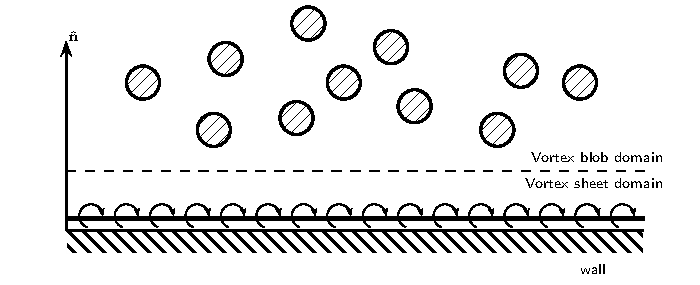
\includegraphics[width=0.8\textwidth]{figures/lagrangian/extendedVorticityField.pdf}
	\caption{Extended vorticity field: Vortex sheet being an extension to the vorticity field (resolved by the vortex blobs) which is able to fully resolve the boundary vorticity}
	\label{fig:extendedVorticityField}
	\end{figure}	
	
When considering a moving boundary, we must also take into account of the circulation of the body due to its motion. The net circulation of the problem is given as
	\begin{equation}
	\Gamma = \Gamma_{\omega} + \Gamma_{\gamma} + \Gamma_{b} = 0,
	\end{equation}	
where $\Gamma_{\omega}$ is the circulation of the vorticity in the fluid (i.e. the vortex blobs), $\Gamma_{\gamma}$ is the wall bounded circulation (i.e. vortex sheets),
	\begin{equation}
	\Gamma_{\gamma} = \oint\limits_S\gamma\left(s\right)\ d s,
	\end{equation}	
and the $\Gamma_b$ is the circulation of the moving body. The circulation inside the body can be considered also be considered as an extension to the vorticity field, where the body is filled with uniform vorticity due to the rotation of the body. Therefore the circulation of a moving body can calculated simply integrating the ``vorticity'' inside the body
	\begin{equation}
	\Gamma_b = \iint\limits_{body} \nabla \times \mathbf{u}_b \ d A.
	\end{equation}	

So the constraint imposed on the net circulation of the vortex sheets is given as,
	\begin{equation}
	\Gamma_{\gamma} = - \left(\Gamma_{\omega} + \Gamma_b\right).
	\end{equation}	

Now, in a pure lagrangian, we must transfer the vorticity generated from the body to the fluid. This is typically done by diffusing the vorticity of the vortex on the fluid, however in our hybrid coupling method, we can use the eulerian domain to introduce the vorticity into the fluid. The eulerian domain acts as the near-wall solver \cite{Daeninck2006}, and the strengths of the particles is interpolated from the eulerian domain, section \ref{}.\todo{CiTe Hybrid sectin}

\subsection{Panel method for treating no-slip boundary condition}
Equation \ref{eq:fredholmIntegral2ndKind} is solved by discretizing the body into $M$ vortex panels giving us a system of equation with can used to determine the $M$ unknowns of the strength of the vortex panels. The method refered as panel method has been greatly summarized by Katz and Plotkin \cite{Katz2001a}. 

Katz and Plotkins have shown several types of panel distributions with various orders of accuracy, from $0^{\mathrm{th}}$
order point vortex or up to $2^{\mathrm{nd}}$ order varying panel strength curvatured distribution. For this project, we have used a constant-strength vortex distribution that discretized the vortex sheet into straight segments, classified as \printAcron{Constant-Strength Vortex Method}{CSVM}.

Panel methods are constructed by discretizing the integral equation and forming a system of equations to solve the $M$ unknowns of the vortex panel,

	\begin{equation}
	\underbrace{\begin{pmatrix}
	-\frac{1}{2} & a_{12} & \cdots & a_{1M}\\ 
	a_{21} & -\frac{1}{2} & \cdots & a_{2M}\\
	\vdots & \vdots & \ddots & \vdots\\ 
	a_{M1} & a_{M2} & \cdots & -\frac{1}{2}
	\end{pmatrix}}_{\mathbf{A}_{MM}} \underbrace{\begin{pmatrix}
	\gamma_{1}\\ \gamma_{2}\\
	\vdots\\
	\gamma_M\\
	\end{pmatrix}}_{\vec{\gamma}} = \underbrace{\begin{pmatrix}
	\mathrm{RHS}_1\\ 
	\mathrm{RHS}_2\\ 
	\vdots\\
	\mathrm{RHS}_M
	\end{pmatrix}}_{\overrightarrow{\mathrm{RHS}}}
	\label{eq:vortexSheetSystemofEquations}
	\end{equation}


where $A_{MM}$ contains the weights of the influence of the vortex panels $\vec{\gamma}$ on each other and the $\overrightarrow{\mathrm{RHS}}$ is

	\begin{equation}
	\mathrm{RHS} = \mathbf{u}_{\mathrm{slip}}\cdot\mathbf{\hat{s}}
	\end{equation}
	
is the boundary condition to the system of equations. In addition, we have another constraint on the net circulation of the vortex panels and in discrete from we say that,

	\begin{equation}
	\sum_{i}^{M} \gamma_i\Delta s = \Gamma_{\gamma}
	\end{equation}	

and results in a $M+1$ system of equations for solving the $M$ unknown strengths of the vortex panels,

	\begin{equation}
	\underbrace{\begin{pmatrix}
	-\frac{1}{2} & a_{12} & \cdots & a_{1M}\\ 
	a_{21} & -\frac{1}{2} & \cdots & a_{2M}\\
	\vdots & \vdots & \ddots & \vdots\\ 
	a_{M1} & a_{M2} & \cdots & -\frac{1}{2}\\
	\Delta s_1 & \Delta s_2 & \cdots & \Delta s_M
	\end{pmatrix}}_{\mathbf{B}_{\left(M+1\right)M}} \underbrace{\begin{pmatrix}
	\gamma_{1}\\ \gamma_{2}\\
	\vdots\\
	\gamma_M\\
	\end{pmatrix}}_{\vec{\gamma}} = \underbrace{\begin{pmatrix}
	\mathrm{RHS}_1\\ 
	\mathrm{RHS}_2\\ 
	\vdots\\
	\mathrm{RHS}_M\\
	\Gamma_{\gamma}
	\end{pmatrix}}_{\overrightarrow{\mathrm{RHS}}}
	\end{equation}

However, as we have an additional constraint on the net strength of the panels, we have $M+1$ set of equations with $M$ unknowns giving us a overdetermined problem. The approach to solve such a problem is either by using a \printAcron{Least-Square solution method}{LSTSQ}, or introducing a new unknown or as used by Katz, eliminating an equation. Enforcing the no-slip boundary condition at each panel location is our vital criteria and therefore, elimination of an equation is not a viable strategy and so the LSTSQ method was utilized for the project.

\subsubsection{Constant-Strength Vortex Method}

The Constant-Strength vortex method ({\color{darkblue}CSVM}) is based on the flat (straight) discretization of the vortex sheet, where the panel have constant vortex strength as per definition. To solve the strengths of the panel problem, we enforce the dirichlet velocity boundary conditions at the collocation point $x_{cp}$, which is located just below the vortex sheet, figure \ref{fig:vortexPanelDefinition}. The coefficient $a_{ij}$ of the influence matrix $\mathbf{A}$ is defined as
	\begin{equation}
	a_{ij} = \mathbf{\hat{u}}_{ij} \cdot \mathbf{\hat{t}}_i,
	\end{equation}
		
and is the tangential influence coefficient of $j^{\mathrm{th}}$ panel on the $i^{\textrm{th}}$ panel. Therefore, induced velocity $\mathbf{\hat{u}}_{ij} = \left(\hat{u},\hat{v}\right)_{ij}$ is the unit induced velocity of the $j^{\mathrm{th}}$ panel on to the collocation points of $i^{\mathrm{th}}$ panel, where the vortex panels have unit strength (i.e $\hat{\gamma}_i = 1$). In general, the induced velocity of the vortex panels are calculated in the local panel coordinates, figure \ref{fig:panelDefinitions}, and the transformation from the local panel coordinate $(x',y')$ to the global coordinates systems $(x,y)$ is given by 

	\begin{equation}
	\begin{bmatrix}
	u_{ij}\\
	v_{ij}\\
	\end{bmatrix} = \begin{bmatrix}
	\cos\alpha_j & \sin\alpha_j \\
	-\sin\alpha_j & \cos\alpha_j
	\end{bmatrix} \cdot \begin{bmatrix}
	u'_{ij}\\
	v'_{ij}
	\end{bmatrix}
	\end{equation}

The induced velocity of the vortex panel $j$ on the collocation point $i$ is given as

	\begin{subequations}
	\begin{align}
	u'_{ij} &= \frac{\gamma_j}{2\pi}\left[\tan^{-1}\frac{y'_i-y'_{j,2}}{x'_i-x'_{j,2}} - \tan^{-1}\frac{y'_i-y'_{j,1}}{x'_i -x'_{j,1}}\right],\\
	v'_{ij} &= -\frac{\gamma_j}{4\pi}\ln\frac{\left(x'_i-x'_{j,1}\right)^2 + \left(y'_i-y'_{j,1}\right)^2}{\left(x'_i-x'_{j,2}\right)^2+\left(y'_i-y'_{j,2}\right)^2}
	\end{align}
	\end{subequations}

\begin{figure}[t]
        \centering
        \begin{subfigure}[b]{0.5\textwidth}
                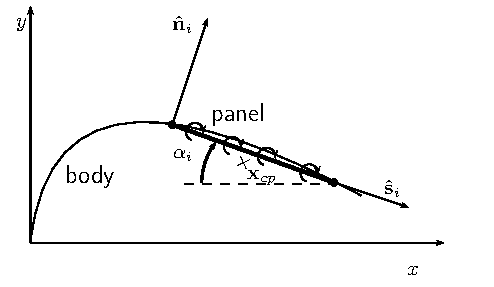
\includegraphics[width=\textwidth]{figures/lagrangian/panelCoordinateDefinition.pdf}
                \caption{Panel discretization of the body in the global cartesian coordinates system $\left(x,y\right)$ and local panel coordinates rotated by $\alpha_i$.}
                \label{fig:panelCoordinateDefinition}
        \end{subfigure}%
        ~ %add desired spacing between images, e. g. ~, \quad, \qquad etc.
          %(or a blank line to force the subfigure onto a new line)
        \begin{subfigure}[b]{0.5\textwidth}
                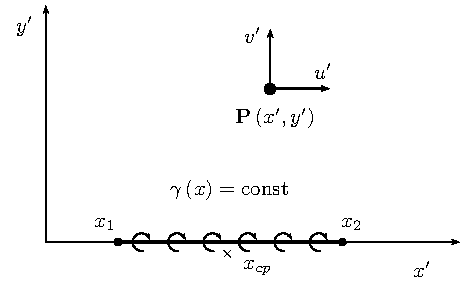
\includegraphics[width=\textwidth]{figures/lagrangian/vortexPanelDefinition.pdf}
                \caption{Constant strength vortex panel in the local panel coordinate system $\left(x',y'\right)$ inducing velocity on the point $P$.}
                \label{fig:vortexPanelDefinition}
        \end{subfigure}
        \caption{Vortex panel's global \textbf{(a)} and local \textbf{(b)} coordinates system definition as defined by Katz and Plotkins \cite{Katz2001a}.}
        \label{fig:panelDefinitions}
\end{figure}	
	
where $(x'_1,y'_1)_j$ and $(x'_2,y'_2)_j$ are the coordinates of the panel start and end point in its local panel coordinate system. Note that the self-induction of the vortex panel (when $i=j$), the influence coefficient becomes $a_{ij} = -1/2$, and can be seen in the diagonal terms of equation \ref{eq:vortexSheetSystemofEquations}. So, by taking $\hat{\gamma}_i = 1$, we are able to construct the influence coefficients of the influence matrix $\mathbf{A}$ and can solve the strengths of the panel, 
	\begin{equation}
	\mathbf{B}\cdot\gamma = \mathrm{RHS},
	\end{equation}
using the LSTSQ method. 

	\begin{figure}[b]
	\centering
	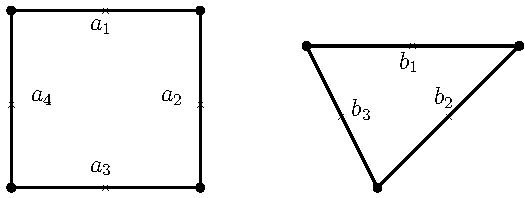
\includegraphics[width=0.6\textwidth]{figures/lagrangian/twoPanelBodies.pdf}
	\caption{twoPanelBodies}
	\label{fig:twoPanelBodies}
	\end{figure}

If we are dealing with multiple geometries, figure \ref{fig:twoPanelBodies}, the panel method can be easily extended by constructing a global influence matrix, 

	\begin{equation}
	\underbrace{\begin{pmatrix}
		c_{a_1a_1} & \cdots & c_{a_1a_N} & c_{a_1b_1} &\cdots & c_{a_1b_M}\\
		\vdots & \ddots & \vdots & \vdots &\ddots & \vdots\\
		c_{a_Na_1} & \cdots & c_{a_Na_N} & c_{a_Nb_1} &\cdots & c_{a_Nb_M}\\
		c_{b_1a_1} & \cdots & c_{b_1a_N} & c_{b_1b_1} &\cdots & c_{b_1b_M}\\
		\vdots & \ddots & \vdots & \vdots &\ddots & \vdots\\
		c_{b_Ma_1} & \cdots & c_{b_Ma_N} & c_{b_Mb_1} &\cdots & c_{b_Mb_M}\\
		\Delta s_{a_1} & \cdots & \Delta s_{a_N} & 0 & \cdots & 0\\
		0 & \cdots & 0 & \Delta s_{b_1} & \cdots & \Delta s_{b_M}\\
	\end{pmatrix}
	\begin{pmatrix}
		\gamma_{a_1}\\
		\vdots\\
		\gamma_{a_N}\\
		\gamma_{b_1}\\
		\vdots\\
		\gamma_{b_M}\\
	\end{pmatrix}}_{\begin{pmatrix}
						AA & AB \\
						BA & BB \\
						\Delta s_A & 0\\
						0 & \Delta s_B \\
					\end{pmatrix} \begin{pmatrix}
								\gamma_{A}\\
								\gamma_{B}\\
							\end{pmatrix}} 
	= 
	\underbrace{\begin{pmatrix}
		\mathrm{RHS}_{a_1}\\
		\vdots\\
		\mathrm{RHS}_{a_N}\\
		\mathrm{RHS}_{b_1}\\
		\vdots\\
		\mathrm{RHS}_{b_M}\\
		\Gamma_{\gamma,a}\\	
	\Gamma_{\gamma,b}
	\end{pmatrix}}_{ 
			\begin{pmatrix}
				\mathrm{RHS}_{a}\\
				\mathrm{RHS}_{b}\\
				\Gamma_{\gamma,a}\\	
				\Gamma_{\gamma,b}
			\end{pmatrix}}
	\end{equation}

where the diagonal matrices ($AA, BB$) are the self-induction matrix of the panel body and the non-diagonal terms ($AB,BA$) are the inter-induction matrix containing the panel influence of $B\rightarrow A$ and $A\rightarrow B$ respectively. The final two rows of the induction matrix contains the additional circulation constraint for each body.


%	\begin{equation}
%	\begin{pmatrix}
%	\mathrm{ab} & \mathrm{ab}\\
%	\mathrm{ba} & \mathrm{bb}\\
%	\Delta s_a & 0\\
%	0 & \Delta s_b
%	\end{pmatrix}
%	\begin{pmatrix}
%	\gamma_a\\
%	\gamma_b	
%	\end{pmatrix} = \begin{pmatrix}
%		\mathrm{RHS}_a\\
%		\mathrm{RHS}_b\\
%		\Gamma_{\gamma,a}\\	
%		\Gamma_{\gamma,b}
%		\end{pmatrix}
%	\end{equation}

%
\subsection{Convergence study of panel method}
The validation of the panel method was done by performing a convergence study of a cylinder. The vortex panels where used to simulate a potential flow around a cylinder and the solution of the panels was compared with the analytical solutions.

	\begin{table}[b]
	    \centering
	    \begin{tabular}{ l r c }
	        \hline
	        Parameters\T\B              & Value 	& Unit    \\
	        \hline
	        $R$\T                     	& $1$	    & $[m\cdot s^{-1}]$ \\
	        $\mathbf{u}_{\infty}$ 		& $\left[1, 0\right]$  	& $[m\cdot s^{-1}]$ \\
	        $N_{\mathrm{panels}}$\B     & $100$  	& $[-]$   \\
	        \hline
	    \end{tabular}
	    \caption{Panel study parameters}
	    \label{tab:panelParams}
	\end{table}

To test the solution of the vortex panels with the analytical solution, the problem was first run for the parameters in the table \ref{tab:panelParams}. The velocity field of the potential flow solution is shown in figure \ref{fig:panelCylinder_velocityField}. The figure shows the norm of the velocity, and we see that it shows the velocity field of a potential flow solution, with an infinitely thin boundary layer, stagnating to zero velocity inside the body.

	\begin{figure}[t]
	\centering
	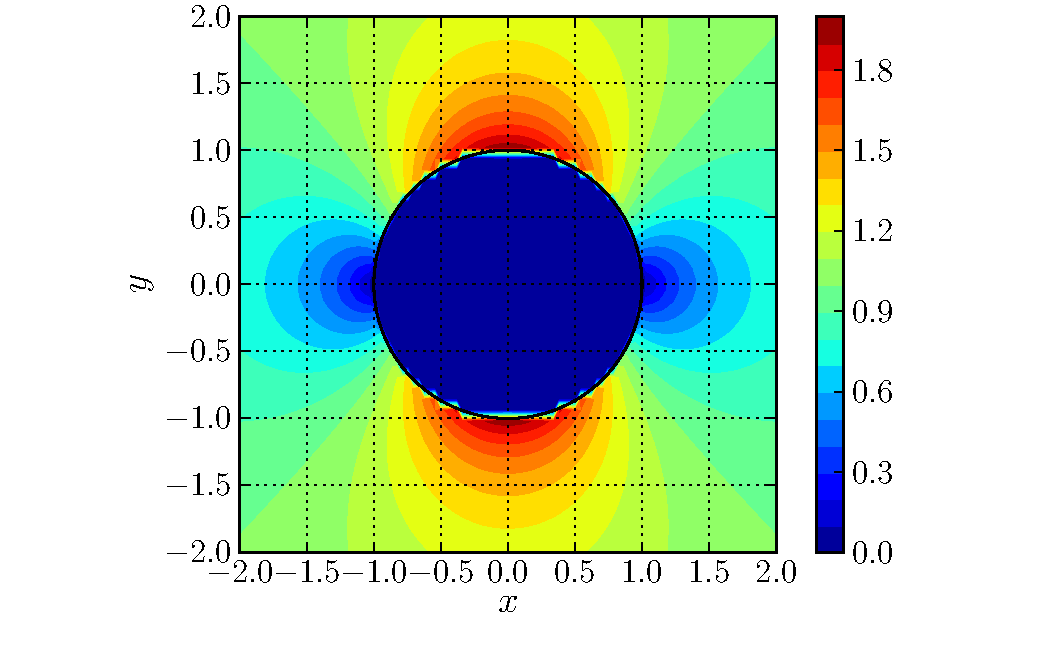
\includegraphics[width=0.7\textwidth]{figures/lagrangian/panelCylinder_velocityField.pdf}
	\caption{Panel method solution: Potential flow velocity field around unit cylinder. The figure depicts $\left\Vert\mathbf{u}\right\Vert$ with zero velocity inside the body.}
	\label{fig:panelCylinder_velocityField}
	\end{figure}

The jagged velocity field around the surface of the cylinder is simply due to the sampling resolution of the field; For higher resolution, this will not be there. In order to determine the accuracy of the solution, the velocity field of the panel solution was compared with the analytical solution. The analytical velocity field around a cylinder is given as,
	\begin{subequations}
	\begin{align}
	u_r &= u\left(1 - \frac{R^2}{r^2}\right)\cos\theta\\
	u_{\theta} &= -u\left(1+\frac{R^2}{r^2}\right)\cos\theta
	\end{align}
	\label{eq:potentialCylinderAnalytical}
	\end{subequations}	
where $u_r$ and $u_{\theta}$ are the radial and the angular velocity respectively. The equation \ref{eq:potentialCylinderAnalytical} is a function of the radius from the center of the cylinder (in our case $r_0 = [0, 0]$) and the radius of the cylinder $R$. 

\begin{figure}[!b]
        \centering
        \begin{subfigure}[b]{0.5\textwidth}
                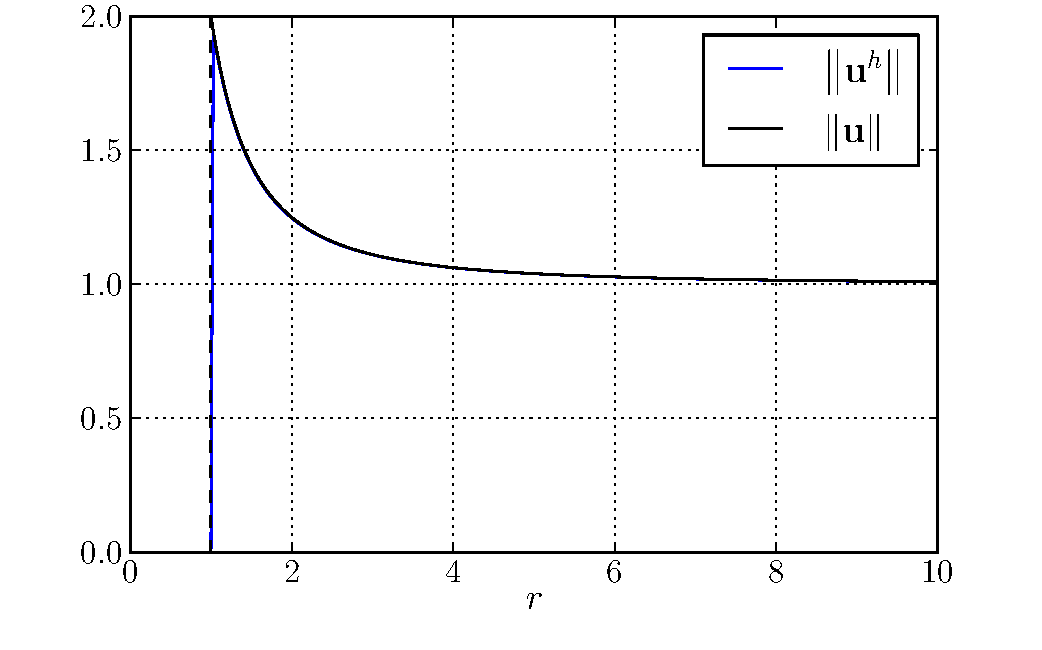
\includegraphics[width=\textwidth]{figures/lagrangian/panelCylinder_versusAnalytical.pdf}
                \caption{Comparison of the velocity field.}
                \label{fig:panelCylinder_versusAnalytical}
        \end{subfigure}%
        ~ %add desired spacing between images, e. g. ~, \quad, \qquad etc.
          %(or a blank line to force the subfigure onto a new line)
        \begin{subfigure}[b]{0.5\textwidth}
                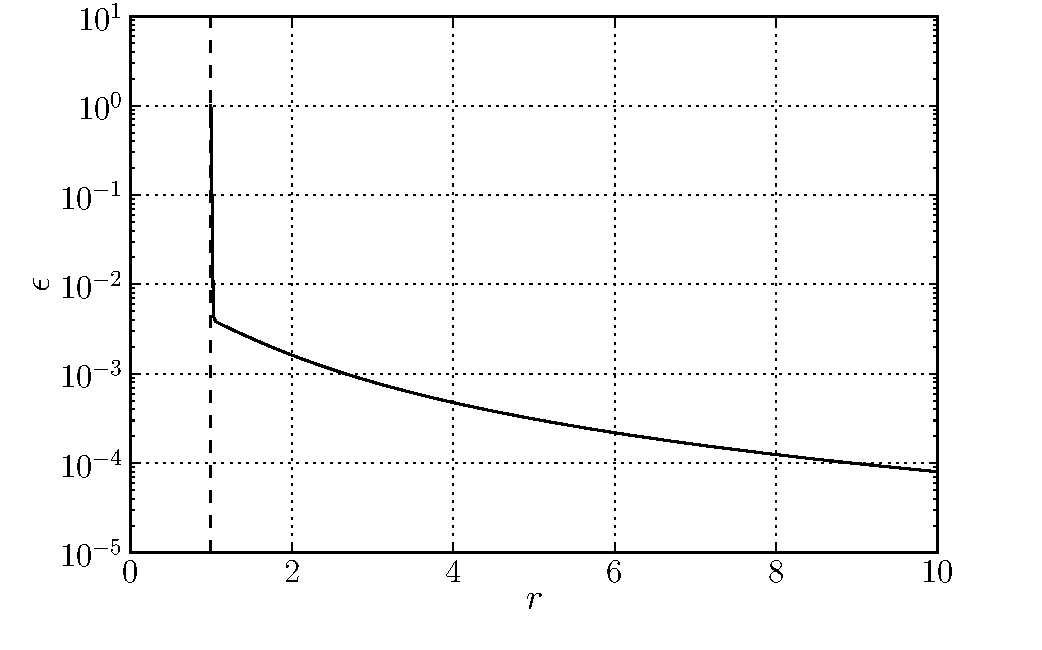
\includegraphics[width=\textwidth]{figures/lagrangian/panelCylinder_error.pdf}
                \caption{Error in velocity field}
                \label{fig:panelCylinder_error}
        \end{subfigure}
        \caption{Comparison of the velocity field along the $y$-axis $0\rightarrow10$. Figure \textbf{(a)} shows both the solutions, the numerical $\left\Vert\mathbf{u}^h\right\Vert$ [solid blue,{\color{plotBlue}{---}}] and the analytical solution [solid black, ---]. Figure \textbf{(b)} shows the relative error $\epsilon$ between the solution, given by equation \ref{eq:panelRelativeError}}
        \label{fig:panelCylinderComparision}
\end{figure}	

The velocity field of the panel was compared with this analytical solution along the y-axis from $y=0$ to $y=10$, figure \ref{fig:panelCylinder_versusAnalytical}. Comparing the solutions of the plot we see that the solution of the vortex panels and the analytical potential flow solution matches everywhere except at the surface. This is correct because the potential flow solution has a slip velocity (i.e non-zero velocity) at the surface of the body, whereas the vortex panels solves for a no-slip boundary condition at the collocation points of the surface. This explains the sudden drop of the velocity from two to zero at the surface.	

The figure \ref{fig:panelCylinder_error} shows the relative error $\epsilon$ between the numerical and the analytical solution,
	\begin{equation}
	\epsilon = \frac{\left\Vert\mathbf{u}-\mathbf{u}^h\right\Vert}{\left\Vert\mathbf{u}\right\Vert}
	\label{eq:panelRelativeError}
	\end{equation}
	
where $\mathbf{u}$ is the analytical solution and the $\mathbf{u}^h$ is the numerical (panel method) solution. Ignoring the solution right at the surface ($r=R$), we see that the error between the numerical and the analytical solution reduces from $\epsilon=5\times10^{-3}\rightarrow 8\times10^{-5}$ as we go from $r=1\rightarrow10$. This behavior of the error tells us that the solution of the constant-strength vortex panels gets more accurate as we go further away from the panels; right next to the panels, we have the largest error. This is because the vortex panels discretizes the body using a first-order approximation (straight panels) and also discretizes the vortex sheet strength using a first-order approximation. 

The convergence analysis of the vortex panels shows that the panels that we are employing is indeed a first-order method as the error converges at $\mathcal{O}\left(N\right)$, figure \ref{fig:panelCylinder_convergence}.


	\begin{figure}[!t]
	\centering
	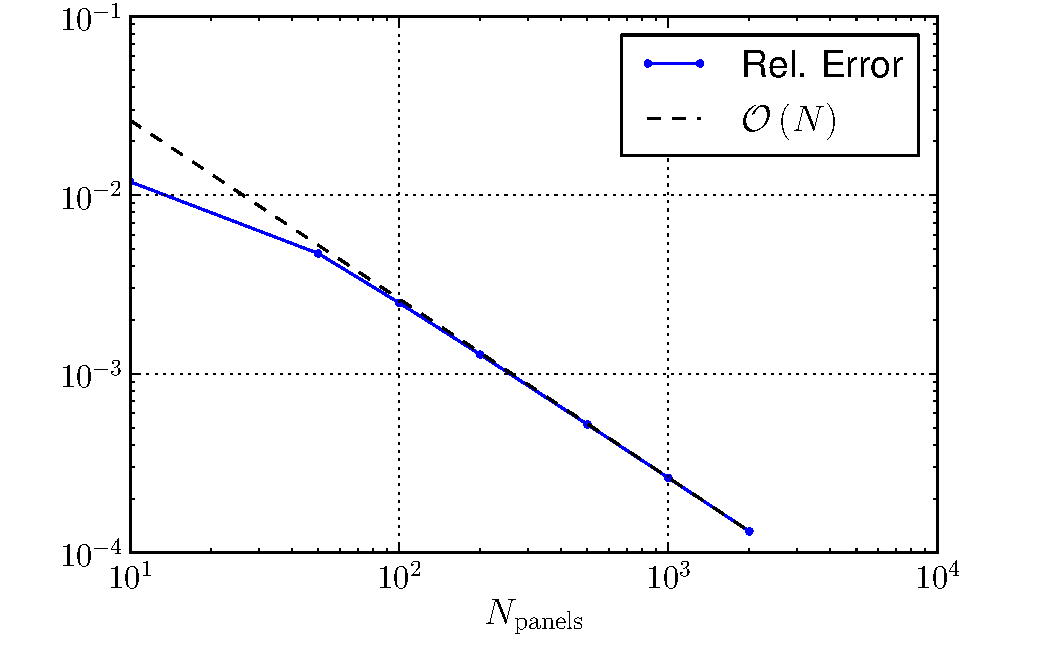
\includegraphics[width=0.7\textwidth]{figures/lagrangian/panelCylinder_convergence.pdf}
	\caption{Convergence plot of the constant-strength straight vortex panels. The figures depicts the reduction is error at $\mathcal{O}\left(N\right)$.}
	\label{fig:panelCylinder_convergence}
	\end{figure}

%\newpage
%\section{Simulation acceleration techniques}
%\label{sec:sat}
%%
%\subsection{Fast multi-pole Method}
%%
%\subsection{Parallel computation in GPU}
%
\section{Validation of lagrangian method}
The validation of the lagrangian method was done by comparing the results of the Lamb-Oseen vortex and the analyzing the convection of the Clercx-Bruneau dipole. Validating each components of the hybrid method separately is vital as to ensure coupling is done correctly.

\subsection{Evolution of Lamb-Oseen vortex}
The evolution of the Lamb-Oseen vortex can be considered to be one of the simplest to validate the viscous vortex method as it is derived from the diffusion equation.

	\begin{figure}[!t]
	\centering
	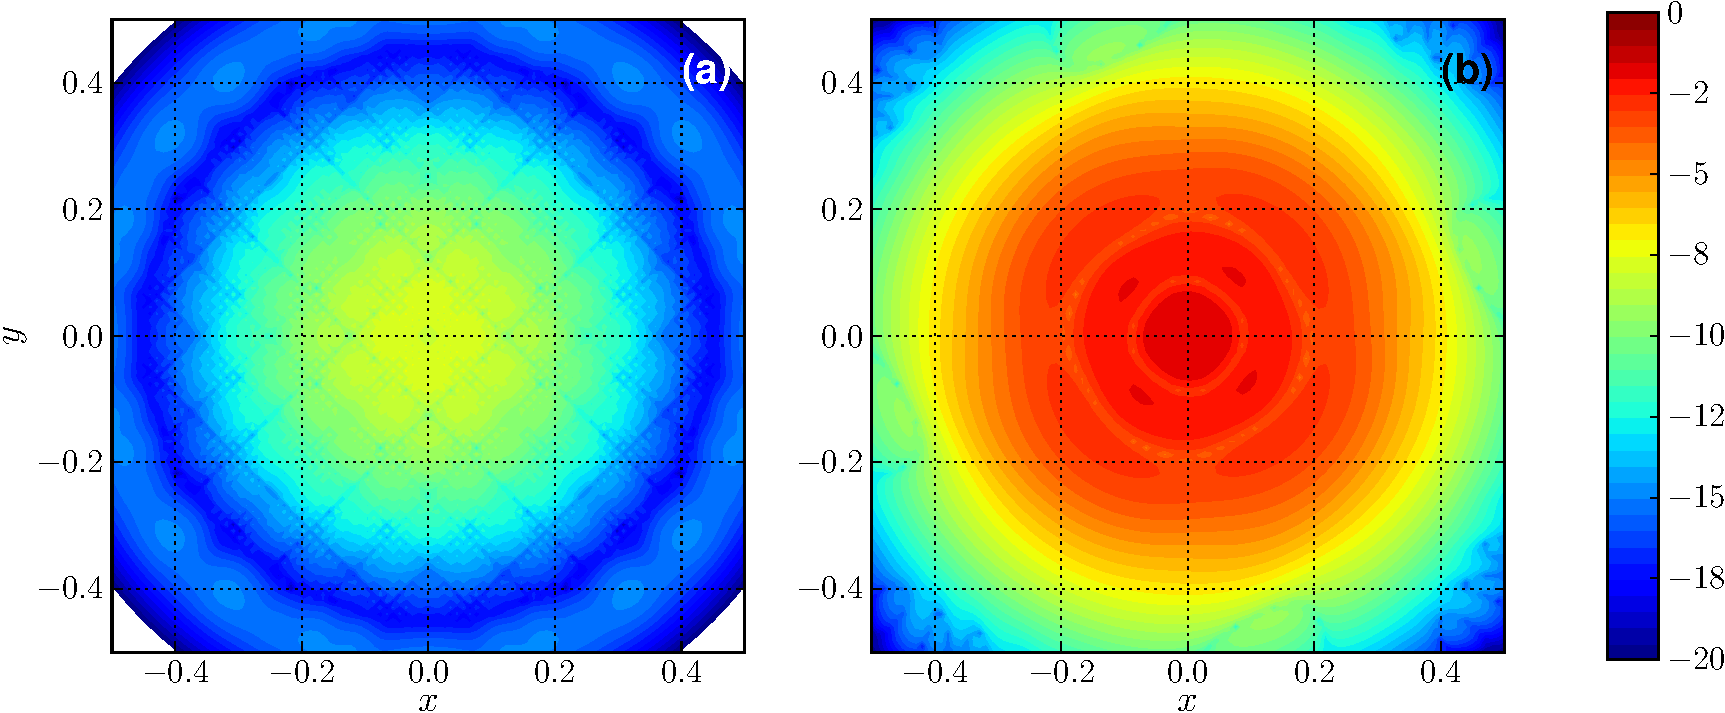
\includegraphics[width=0.99\textwidth]{figures/lagrangian/lambOseen_convection_vorticityErrorContours_compressed-crop.pdf}
	\caption{Error growth of Lamb-Oseen vortex during the evolution}
	\label{fig:lambOseen_convection_vorticityErrorContours_compressed}
	\end{figure}

	\begin{figure}[p]
	\centering
	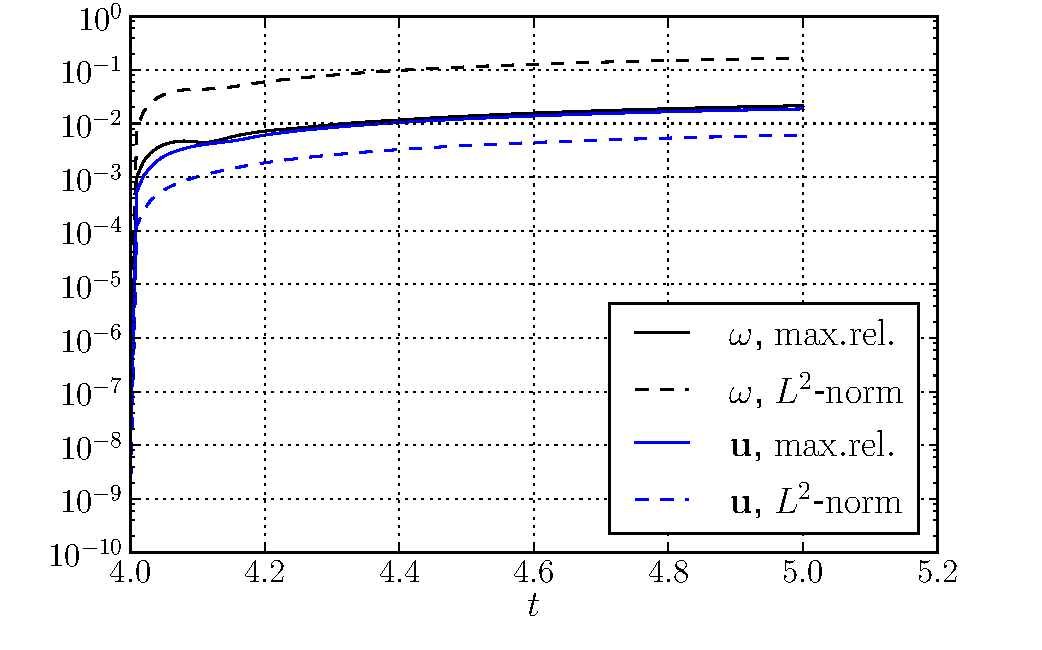
\includegraphics[width=0.7\textwidth]{figures/lagrangian/lambOseen_convection_errorGrowth_compressed.pdf}
	\caption{Error growth of Lamb-Oseen vortex during the evolution}
	\label{fig:lambOseen_convection_errorGrowth_compressed}
	\end{figure}
	
	\begin{figure}[p]
	        \centering
	        \begin{subfigure}[b]{0.5\textwidth}
	                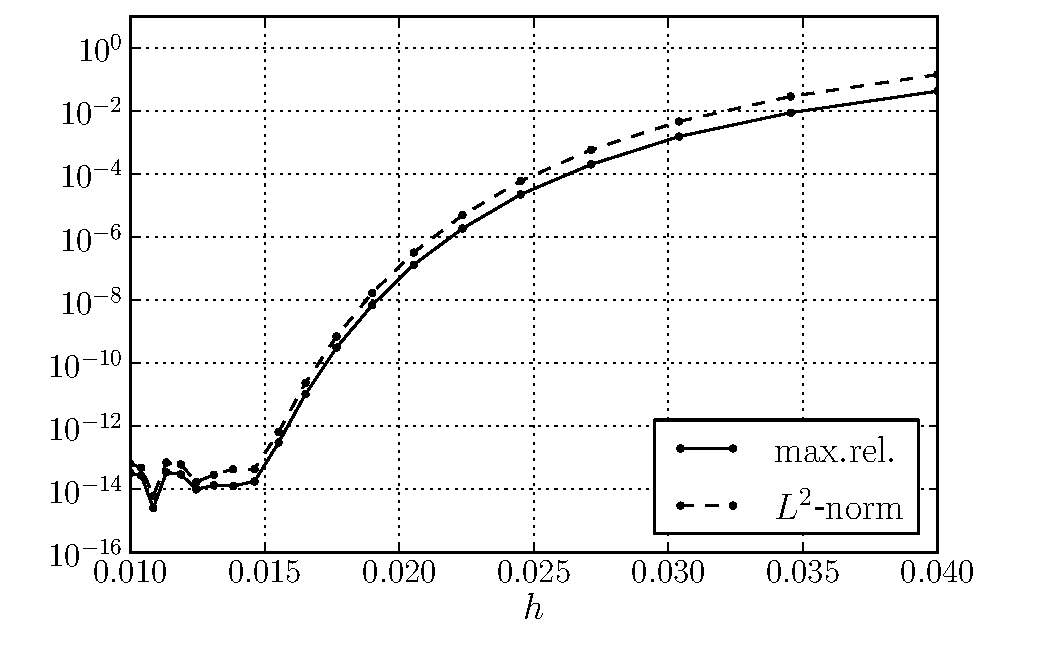
\includegraphics[width=\textwidth]{figures/lagrangian/lambOseen_convergence_dx_sigma0p02_compressed.pdf}
	                \caption{Comparison of the velocity field.}
	                \label{fig:lambOseen_convergence_dx_sigma0p02_compressed}
	        \end{subfigure}%
	        ~ %add desired spacing between images, e. g. ~, \quad, \qquad etc.
	          %(or a blank line to force the subfigure onto a new line)
	        \begin{subfigure}[b]{0.5\textwidth}
	                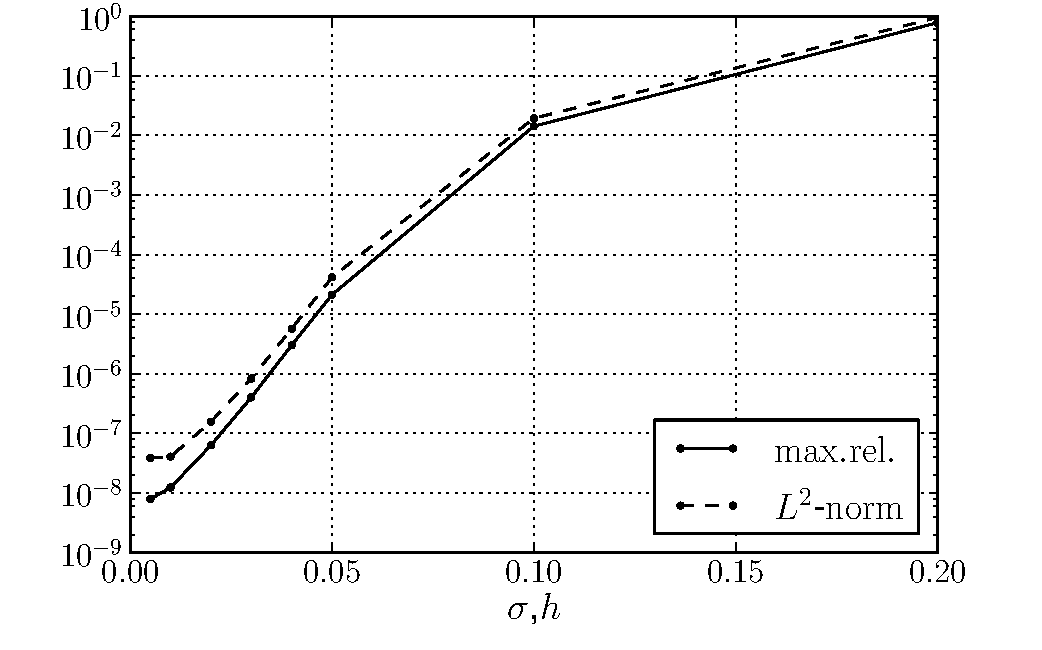
\includegraphics[width=\textwidth]{figures/lagrangian/lambOseen_convergence_dx_compressed.pdf}
	                \caption{Error in velocity field}
	                \label{fig:lambOseen_convergence_dx_compressed}
	        \end{subfigure}
	        \caption{dx}
	        \label{fig:lambOseen_convergence_dx}
	\end{figure}	

	\begin{figure}[p]
	\centering
	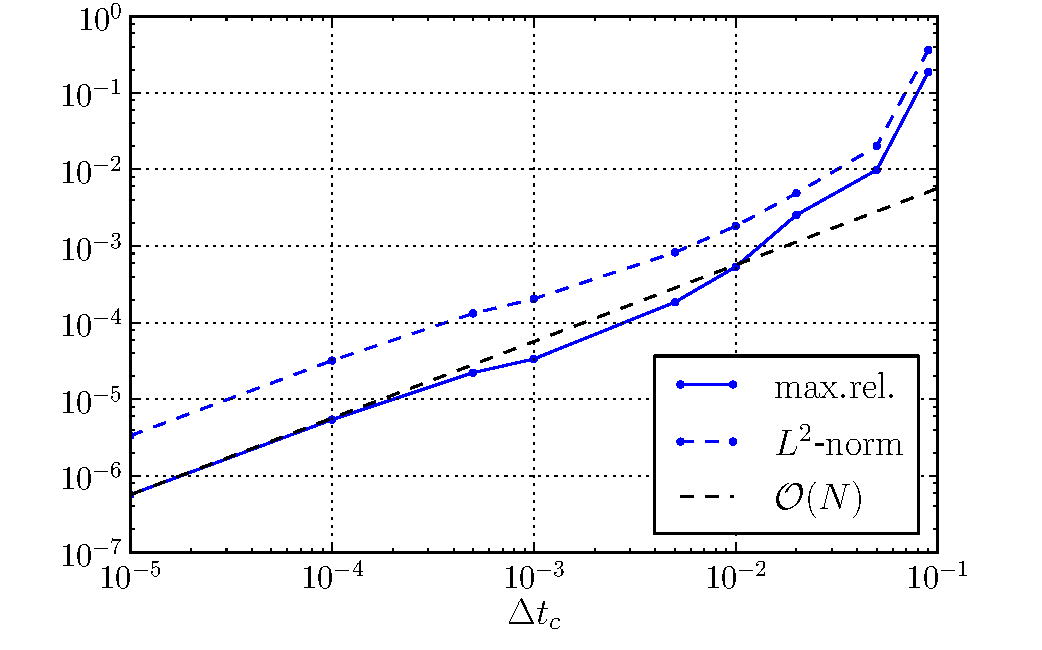
\includegraphics[width=0.7\textwidth]{figures/lagrangian/lambOseen_convergence_dt_compressed.pdf}
	\caption{Error growth of Lamb-Oseen vortex during the evolution}
	\label{fig:lambOseen_convergence_dt_compressed}
	\end{figure}


\subsection{Convergence study of the viscous vortex method}

%%------------------------------------------------------------------------------------------------------
%%------------------------------------------------------------------------------------------------------
%%------------------------------------------------------------------------------------------------------
%
\subsection{Convection of Clercx-Bruneau dipole at $Re=625$}
%
\section{Summary}
%
